\chapter{Catastrophic Forgetting in Hopfield Networks}
\label{chap:SolutionsCF}

Although usually explored using MLP networks, catastrophic forgetting (CF) can be just as easily demonstrated in Hopfield type networks, as is the case in \citet{Robins1998}. However there are a greater variety of causes for catastrophic forgetting in Hopfield networks depending on the learning algorithm and the types of patterns that are learnt.

\begin{figure}[tbp]
  \center
	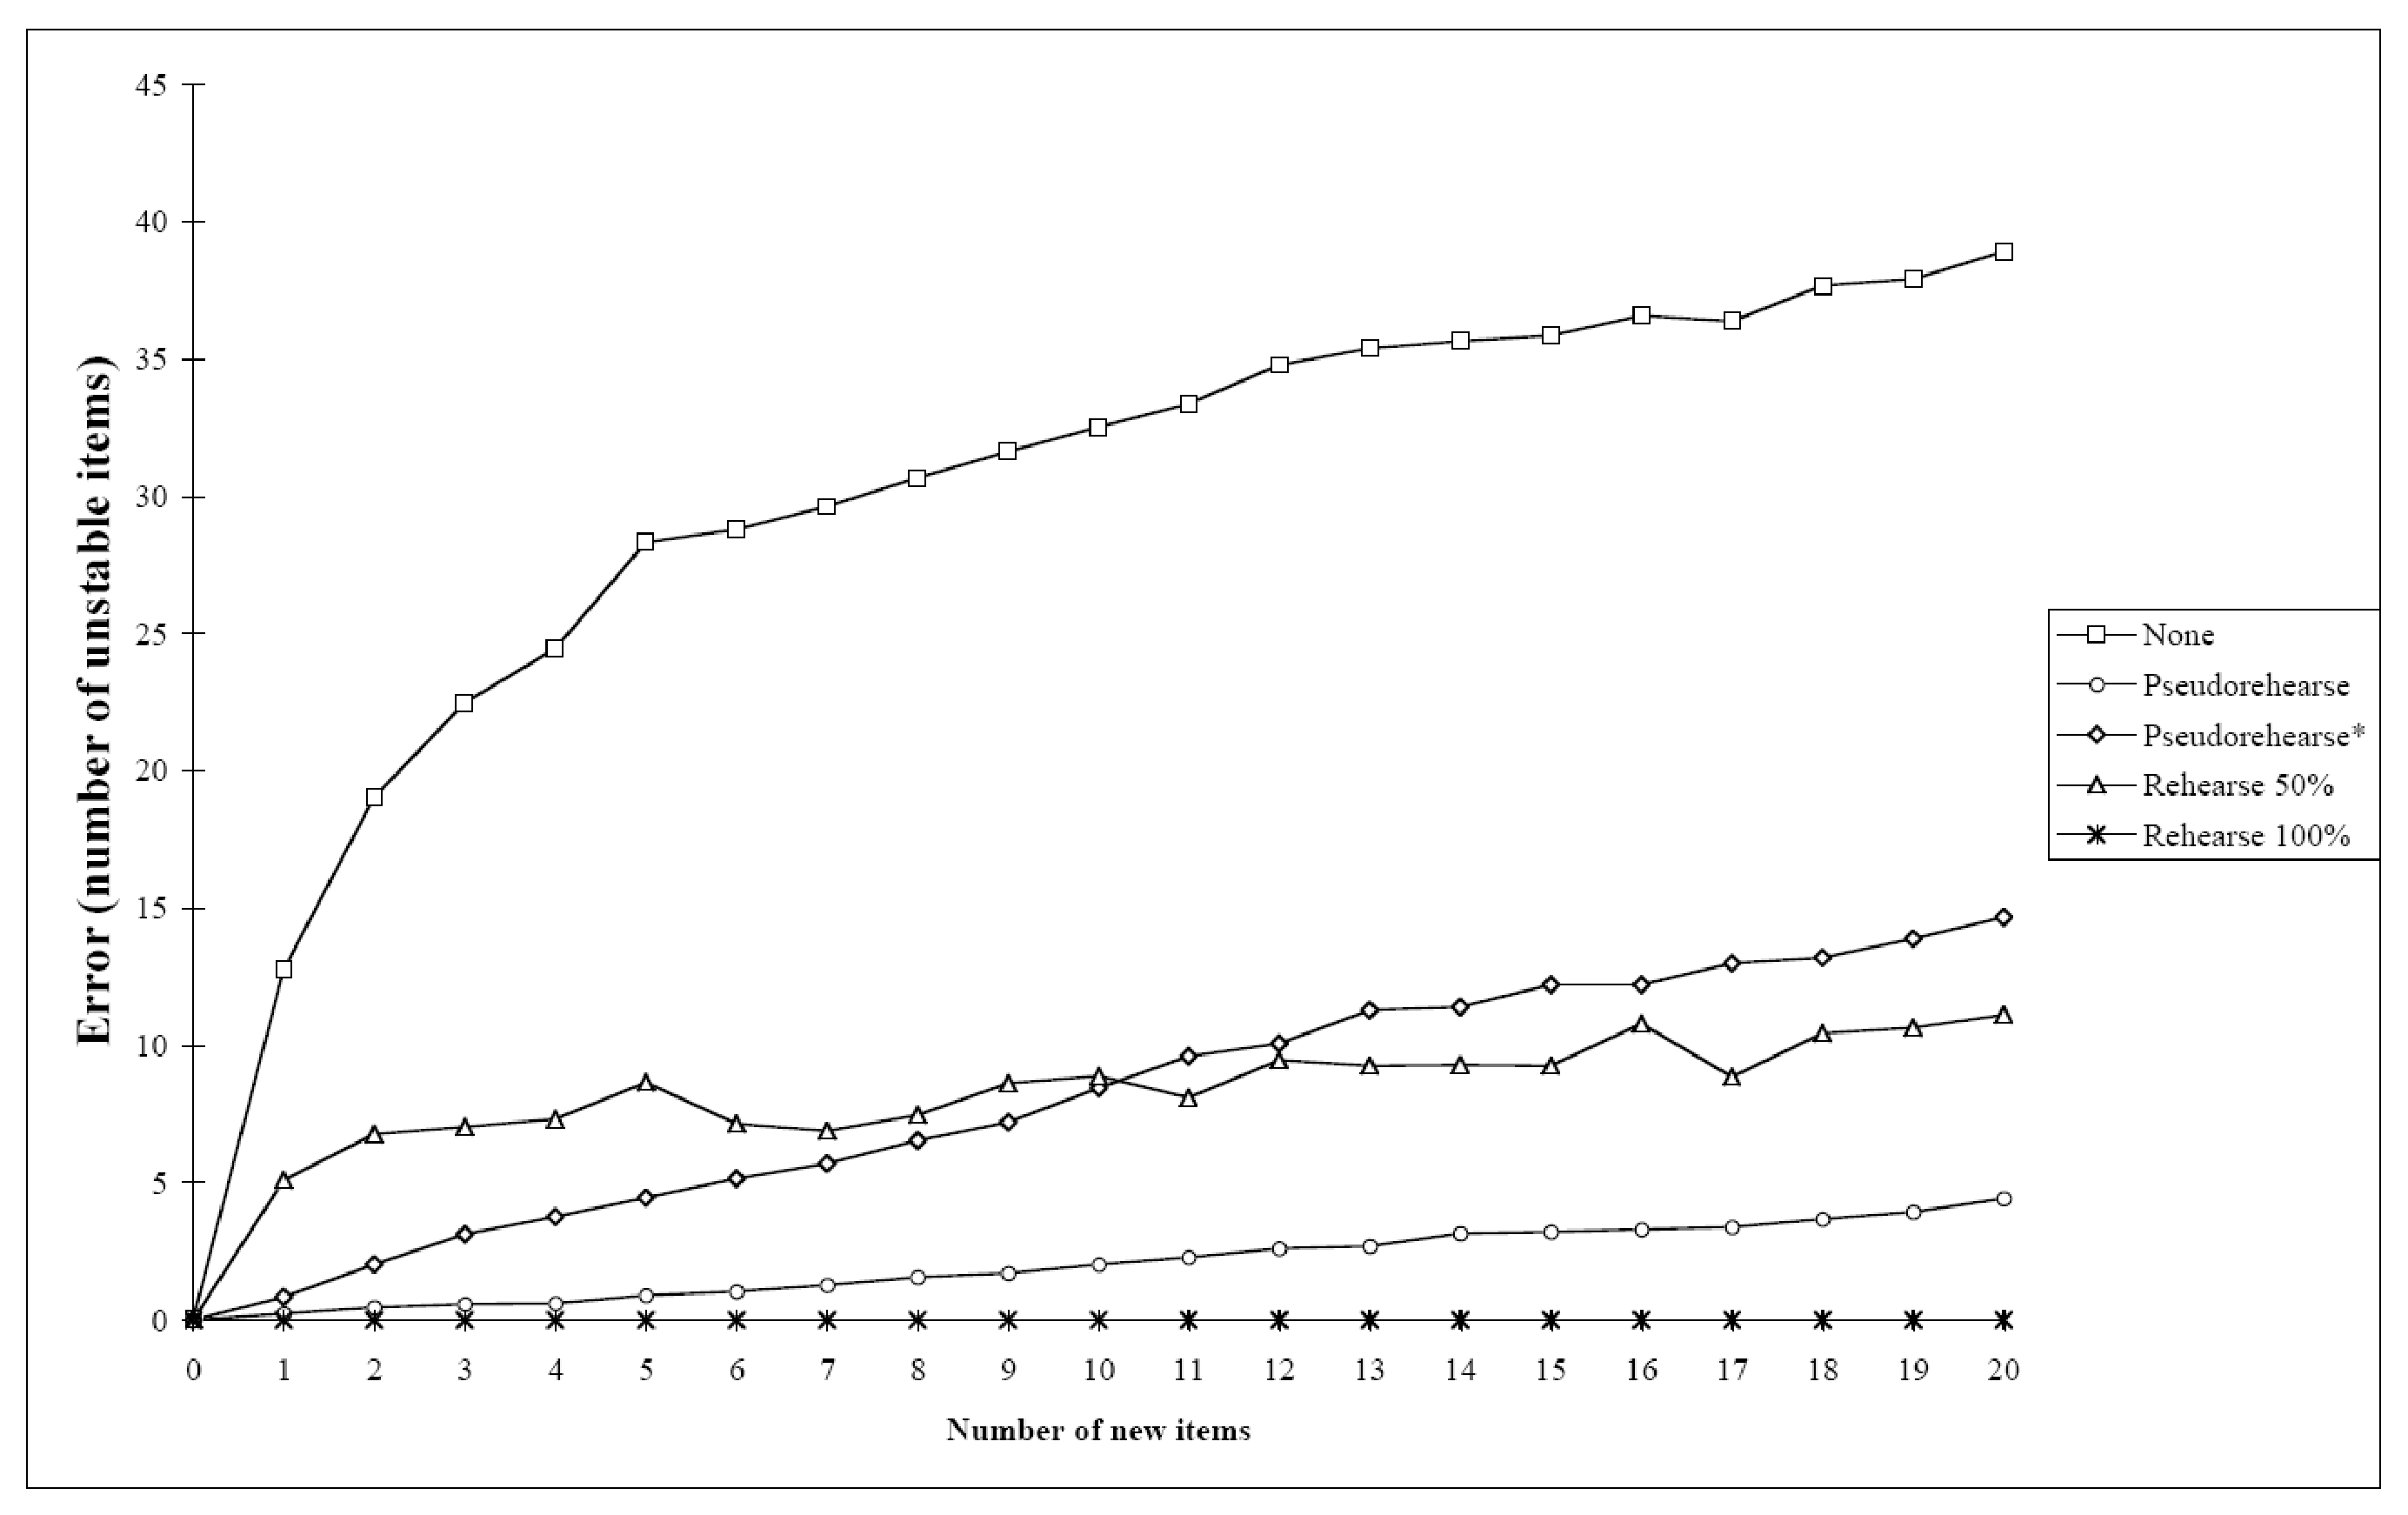
\includegraphics[width=0.90\textwidth]{Figures/HOP-CF.eps}
	\caption{Catastrophic forgetting in an \hopnet{64,\pm}{} network caused by delta learning's excessive plasticity.  Base population of 44 items with 20 new items learnt sequentially (adapted from \citet{Robins1999} Fig 1.).}
	\label{fig:CF-Hop}
\end{figure}

Figure~\ref{fig:CF-Hop} summarises data which illustrates CF as described in Robins and McCallum (1999, Fig 1.). The network is trained on a base population of 44 items so that every item is stable. If the network is then trained in the same way on a single new item, the number of unstable patterns in the base population increases dramatically. This is illustrated in the ``None'' condition of Figure~\ref{fig:CF-Hop} (with no intervention to manage CF). The error continues to increase rapidly as further new items are learnt, and eventually the base population is effectively wiped out. Similar issues have been explored using Hopfield networks by \citet{Nadal1986} and \citet{Burgess1991}, and in the context of the ``unlearning'' mechanisms detailed in Section~\ref{sec:simpleUnlearning}.

When considering the causes of CF in Hopfield networks the capacity of the network is often the first and most obvious issue.  The Hebbian learning algorithm generates CF near the capacity of the network, at which point, if more patterns are learnt, all information both old and new is lost.  We will discuss the capacity, both in terms of the theoretical information capacity and the capacity of particular learning algorithms~\citep{Gardner1988}.


\section{Catastrophic Capacity}
\label{sec:CatastrophicCapacitySol}

Hopfield networks have a relatively low capacity compared to the MLP networks presented earlier, partly because they do not have the additional internal machinery of hidden units.  Adding units to a Hopfield network adds complexity to the problem as \emph{all} units are both inputs and outputs.  Without hidden units it is not possible to just increase the resources available to the learning algorithm by adding units.  Thus the capacity of a Hopfield network is directly proportional to the number of units in the network.

The number of patterns that can be learnt by a Hopfield network is limited by the amount of information that can be stored in the network.  A set of patterns can contain differing amounts of information.  Patterns that have only a single unit active contain less information than a set of patterns where the units are active 50\% of the time.  Randomly generated patterns contain a large amount of information as estimated using either Kolmogorov complexity or Shannon information therory (for and indepth coverage of information therory see \citet{Cover1991}). Information based on probability theory in this context can be described as, how surprising an activation of a unit is, given the previous set of patterns.  With only a single unit active $N-2$ units remain in exactly the same configuration as the previous pattern, and so there is little surprise and thus little information.

For binary units the maximum amount of information is where each pattern has $50\%$ of its units active.  In this thesis all patterns are randomly generated with each unit have a $50\%$ chance of being active.  Some patterns have a coding ratio (ratio of active unit to inactive units) of above or below 50\%.  This type of pattern is used for experiments in the rest of this thesis, unless otherwise stated.

Section \ref{sec:capacity} discussed the capacity of a Hopfield network and presented the estimate of $0.14N$ as a rough upper bound for Hebbian learning. Above this value Hebbian learning shows a particularly severe form of CF where rather than losing just the old material the network can spontaneously lose all stored patterns including the new items.  This can be caused by a single large spurious attractor taking over the whole space with a massive basin of attraction, or by the generation of thousands of small attractors (stable states with a basin of attraction).  When developing solutions to CF in Hopfield networks it is important to evaluate them in networks which are far from capacity as well as those which are close to their theoretical limits.

The catastrophic loss of pattern stability is shown in Figure~\ref{fig:hebb64clean} for a network of 100 units.  The line shows the average over 100 repetitions with error bars extending to one standard deviation. This network shows classic CF under the pressure of capacity.  The storage of this $100$ unit network \(\hopnet{100,\pm}{}\) from equation~\ref{eq:HopnetcapHebbian} is approximately 14 patterns.  Note that by the time 18 patterns have been presented the likelihood of a learnt pattern being stable is about $50\%$ (9 patterns are stable on average).  As more patterns are presented fewer and fewer of them remain stable in the network.  

\begin{figure}[tbp]
\small
\center
	\begin{center}
		\input{Figures/Hebbian/HopCF.tex}
	\end{center}
	\caption{Number of learnt patterns stable in a 100 unit Hopfield network \hopnet{100,\pm}{} with Hebbian learning showing CF (averaged over $100$ repetitions, 50\% random patterns).}
	\label{fig:hebb64clean}
\end{figure}

\section{Catastrophic Correlation}
\label{sec:CatastrophicCorrelation}
Most of the capacity measures for Hopfield networks involve the analysis of uncorrelated random patterns (independent identically distributed random variables -- i.i.d.).  Assuming that all the patterns that need to be learnt will come from these sorts of clean distributions is unrealistic.  Patterns from real data sets are likely to have correlations, and in fact it is likely that it is the correlations between events that makes it possible to extract causal relationships.  Correlations alter the analysis of capacity: 1) the maximum theoretical capacity increases in relation to the amount of overlap and the nature of the correlation~\citep{Gardner1988, Lowe1998, Gandolfo1999, Kimoto2002, Bogacz2003}, and 2) Hebbian learning performs poorly with correlated patterns as the crosstalk term becomes very large and the pattern which is the correlation between inputs becomes the only stable attractor.

To understand why correlation increases the number of patterns that can be stored, the amount of information in each pattern must be analysed.  In the extreme case of only one unit being active in each pattern it is easy to see how to store any of the $N$ ``one unit active'' patterns.  To store these patterns the connections between units are set to a negative value so that active units tend to deactivate other units, and the unit that is active in a pattern has a positive connection from the bias unit so that if it is active it remains active.  This easy solution for storing $N$ patterns is a result of each pattern only having a small amount of information.  Because of the symmetry in binary activation, patterns with all but one unit active contain the same amount of information as patterns with only a single unit active.  

\citet{Amit1987b} argue that Hebbian learning can be altered to accommodate correlated patterns where the correlation is caused by a low coding ratio (only a small percentage of the units are active).  The learning rule can be changed to:
\begin{equation}
	\label{eq:HebbianlearningCorrellated}
	\delta\weight{ij} = (\unitActivation{i}{}-\alpha)(\unitActivation{j}{}-\alpha)
\end{equation}
where $\alpha$ is the sparseness of the coding.  This concept of correlation caused by a uniform decrease in the number of units that are active is useful only when the patterns have a known activity level and that activity level is the {\em only} correlation between the learnt patterns.  The patterns themselves need to be uncorrelated in terms of which units are active for this approach to work.

Correlation does not come from just a change in the coding ratio for the patterns.  One interpretation for correlated patterns is the concept of a prototype.  The prototypical car will have many features in common with individual cars.  A learning set that contains groups of similar objects will have correlated patterns and the combination of these correlations may be the prototype for the group.  

Hopfield networks with Hebbian learning cannot make highly correlated pattern stable.  Instead a pattern which is the combination of the learnt patterns will become a stable state with a large basin of attraction.  There are two types of correlation, one caused by a low coding ratio where the patterns are still independent, and correlation caused by patterns which share a large number of features. The difference can be most clearly demonstrated with an example. 

In this example the learning population is generated by making small perturbations of a checkerboard pattern (Figure~\ref{fig:checkerpert}).  These patterns have a coding ratio of about $50\%$ but are also extremely highly correlated.  This form of correlation immediately destroys the basin of attraction of the individual patterns and the only attractor is the correlated prototype, in this case a checkerboard pattern.  To show this, consider three patterns that are based on a checkerboard pattern with $k$ units altered $(k<<N)$ with alteration ratio ($\alpha_{a}$) $= k/N$ .  Having learnt three patterns there are four catagories of units representing the different types of overlap of the perturbed checkerboard patterns.  The average number of units in each set (cardinality C), can be calcuated from the alteration ration $\alpha_{a}$
\begin{enumerate}
\item The set of units altered in all three patterns. \\
  \hspace{1cm}$\Phi^{3}_{3}=\phi_{1\wedge2\wedge3}$, \\
  \hspace{1cm}$C = \alpha_{a}^3$
\item Units altered in two of the three patterns. \\
  \hspace{1cm}$\Phi^{3}_{2}=\phi_{1\wedge2}+\phi_{2\wedge3}+\phi_{1\wedge3} -
  \phi_{1\wedge2\wedge3}$, \\ 
  \hspace{1cm}$C = 3*(\alpha_{a}^2*(1-\alpha_{a}))$
\item The set of units altered in just one pattern. \\
  \hspace{1cm}$\Phi^{3}_{1}=(\phi_{1} +\phi_{2} + \phi_{3})   
  -(\phi_{1\wedge2}+\phi_{2\wedge3}+\phi_{1\wedge3}+\phi_{1\wedge2\wedge3})$, \\
  \hspace{1cm}$C = 3*(\alpha_{a}*(1-\alpha_{a})^2)$
\item The set of units that conform to the checker board in every learnt pattern.\\
  \hspace{1cm}$\Phi^{3}_{0}=N-\phi_{1\vee 2\vee 3}$, \\
  \hspace{1cm}$C = (1-\alpha_{a})^3$
\end{enumerate}
where $\phi_{1\wedge2\wedge3}$ is the set of units whose activation was altered in all the patterns 1, 2 and 3;
 $\phi_{1\wedge2}$ is the set of units altered in patterns 1 and 2;
 $\phi_{1}$ is the set of units altered in patterns 1; and
 $\phi_{1\vee2\vee3}$ is the set of units altered in pattern 1, 2 or 3.

\begin{figure}[tbp]
\small
\center
	\begin{center}
		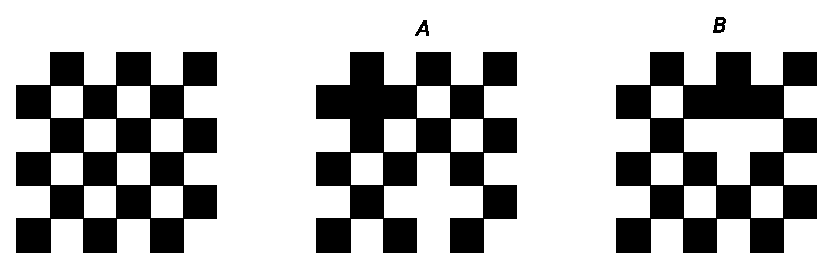
\includegraphics{Figures/checkerboard.eps}
	\end{center}
	\caption{Checker board with two possible perturbations $A$ and $B$.}
	\label{fig:checkerpert}
\end{figure}

If the altered units are selected from an i.d.d.\ at random then $\Phi^3_{3}$ would have cardinality $\approx \alpha_{a}^3*N$.  Given small $k$, the number of units altered in more than one pattern is very small.  A unit $i$ selected at random from the set of units in $\Phi^{3}_{1}$ will have connections to units $j$ in $\Phi^{3}_{0}$, each with a weight $\weight{ij}=1$ giving a net input to the unit of $N*((1-\alpha_{a})^3)$.  Given that the units in the other categories have at most $\weight{ij} = \pm3$ so long as $\alpha_{a} < 0.14$ for three patterns and $\alpha_{a} < 0.22$ for four patterns, the unit will change state to match the checker board.  The more patterns which are learnt from the set of patterns with minor alterations to the checker board pattern, the larger the prototype's basin of attraction becomes.  


If the units in the pattern are slowly ``fatigued'', where their input is lowered by a set amount, after several iterations individual patterns emerge from the prototype. This is because the units that were altered in the learnt patterns are closer to threshold than the units that are only in the checker board pattern.  The major problem with this is that the patterns generated by this process of fatiguing the units are not just the learnt patterns, but include many spurious patterns.


\section{Catastrophic Plasticity}
\label{sec:CP}
Catastrophic forgetting in Hopfield networks with Hebbian learning is mainly attributable to capacity and correlations.  However by using delta learning both the catastrophic correlation and catastrophic capacity problems  are reduced.  Delta learning deals with correlation by only making changes that improve performance, and the capacity is increased dramatically to close to the theoretical information capacity of the network.  

However delta learning in Hopfield networks also suffers from excessive plasticity.  Delta learning is able to learn a larger number of patterns by slowly adjusting the weights until they make the current set of patterns stable.  Thus when learning new patterns, all the weights are changed to match the new patterns.  This plasticity, the key to the power of the learning algorithm, can cause catastrophic forgetting.
 
As discussed in \citet{Robins1998} there is a great deal of similarity between the CF caused by excessive plasticity in MLP networks and in Hopfield networks using delta learning. Figure~\ref{fig:HOP-CP} shows the number of base population patterns that become unstable as new patterns are learnt.  It is this type of CF that is the target of the pseudorehearsal solution presented below in Section~\ref{sec:PRSolution}.

\begin{figure}[tbp]
\small
\center
		 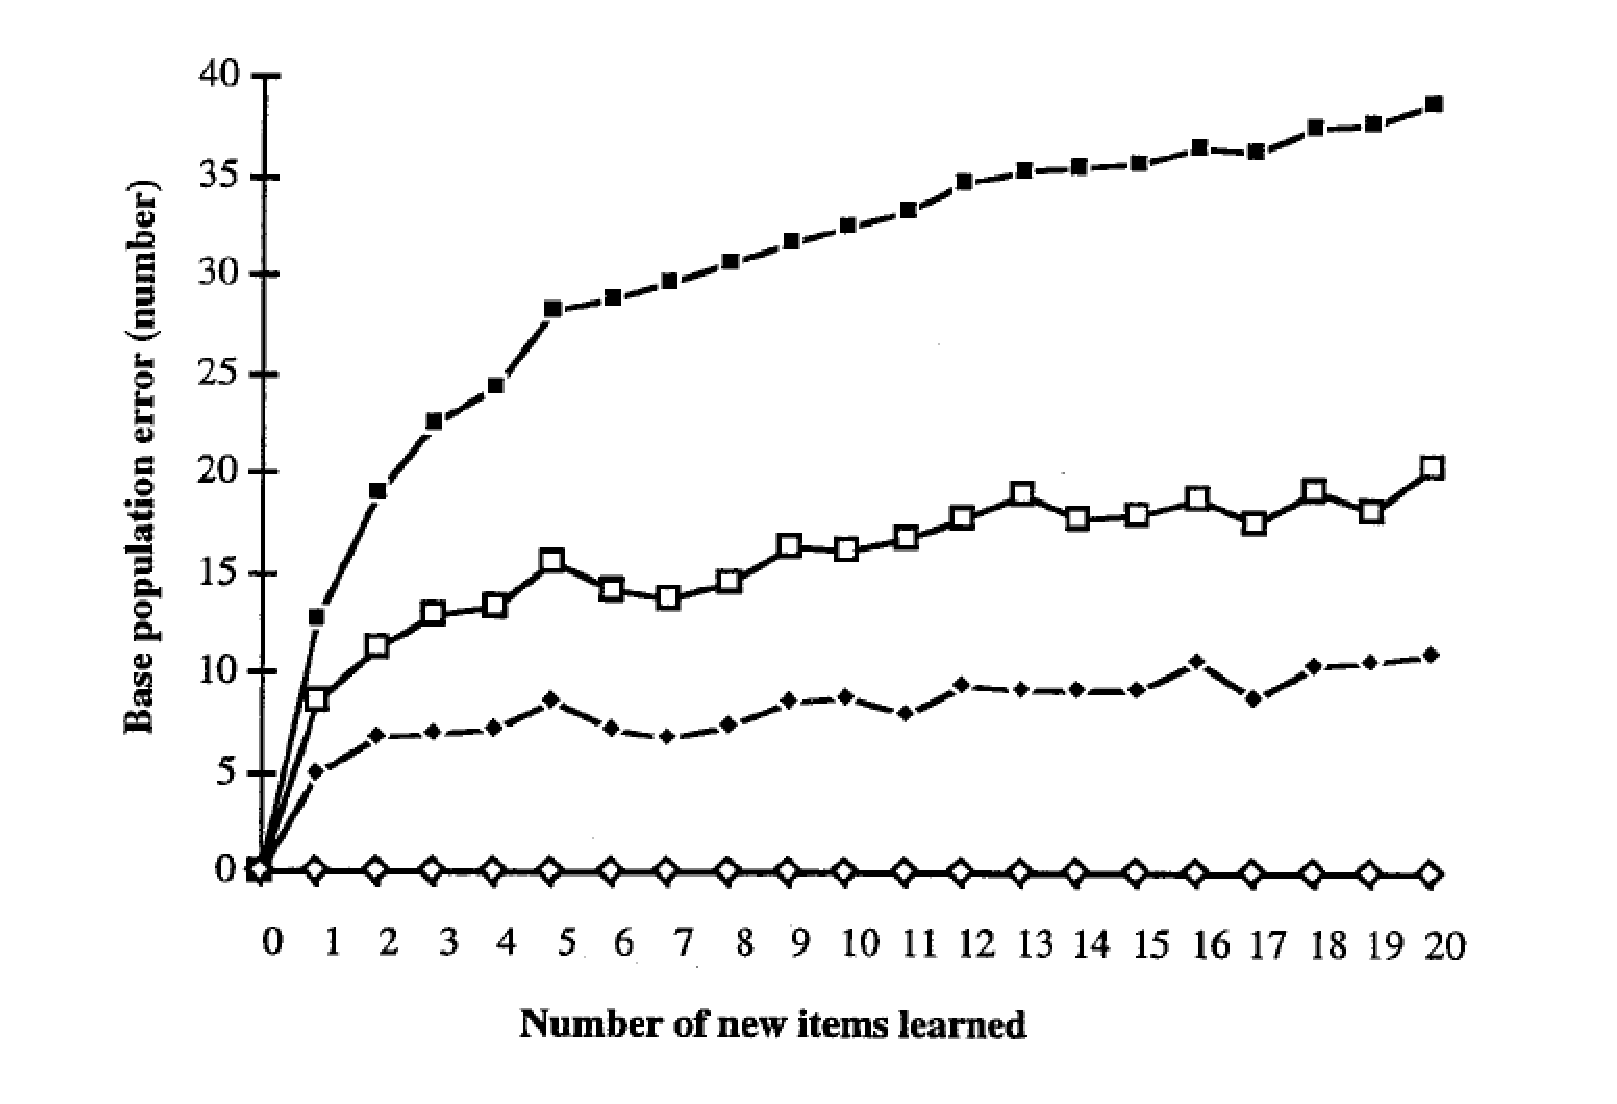
\includegraphics[width=0.90\textwidth]{Figures/HOP-CP.eps} %\input{Figures/HOP-CP} %
	\caption{Catastrophic forgetting in a Hopfield network caused by plasticity (adapted from Robins and McCallum (1998) Figure 4).}
	\label{fig:HOP-CP}
\end{figure}

\section{Existing Solutions}
\label{sec:existingSolutions}

Catastrophic forgetting does not have a single cause, and although the various solutions tend to focus on a particular cause, they usually have an affect on all of the causes.  For example, the unlearning solution (see Section~\ref{sec:simpleUnlearning} was initially designed to solve the problem of the limited capacity of Hopfield networks, and was later analysed to show that it was also affecting the problem of catastrophic correlation~\citep{Christos96}.  The complexity in the interactions between the solutions and the various types of problems makes it difficult to directly compare solutions.  Each solution makes trade-offs between plasticity and stability, complexity and robustness, and biological plausibility.  

One method for dissecting these solutions is to organise them by the level at which they operate. The levels that we define are:
\begin{itemize}[topsep=1ex, leftmargin=1cm, labelsep=0.2cm, itemindent=0pt,label=\textbullet]
  \item Synaptic Level
  \item Neuron Level
  \item System Level
\end{itemize}

In the rest of this chapter we review the existing solutions to CF and place them into this taxonomy, as well as presenting our own pseudorehearsal solution.  The goal of breaking the solutions into these categories is to establish a comparison matrix so that solutions can be compared by complexity and level rather than just raw performance.  A system that requires a much more elaborate control mechanism must perform significantly better than the simplest solution to be considered an improvement.  The performance of some system level solutions can be mainly attributed to the effect of an associated synaptic level alteration.  By analysing the level at which a solution operates we can use a combination of performance and complexity to compare results.


\subsection{Synapse Level}
The synaptic level solutions focus on changing the way in which synaptic updates are performed given local information.  In this section we include systems that either alter the way in which the local update rule is applied to the synapses, or use a post--processing phase to alter the weight matrix after a pattern has been learnt.

\subsubsection{Weight decay}

Weight decay is one of the simplest post--processing operations to implement.  After each item, or set of items, are learnt every weight in the network is multiplied by a value just less than 1.  This reduces the magnitude of each weight, moving it closer to 0.  As Hebbian learning alters the weights by a fixed amount, it is easier to learn a new pattern when the weights are small.   There is also biological evidence of a decay mechanism which reduces and even eliminates connections over time.  There appears to be two types of LTP(long term potentiation), decremental and persistent~\citep{Abraham2003}.  Hebbian learning with weight decay would be equivalent to decremental LTP.  

This can be considered a form of \term{managed forgetting}, where the forgetting of previous information is included in the learning algorithm.  Using weight decay it is possible to calculate the influence on each weight that an old learnt pattern will have, directly from the number of patterns that have been learnt since it was presented.  With weight decay of $\weightDecay = 0.1$ after 10 additional patterns have been learnt, the contribution of the original pattern will be $0.9^{10} = 0.35$ of that pattern's original contribution.  This controlled forgetting allows weight decay to avoid CF. 

\citet{Christos96} showed that weight decay is able to reduce the CF caused by overloading the network, at the cost of lowering the effective capacity to $0.05N$.  Figure~\ref{fig:WeightDecay100num} shows our comparison between normal Hebbian learning and learning with a weight decay of $\weightDecay = 0.1$. The weights are each new pattern are altered so that $( w_{ij} = w_{ij}*(1-\weightDecay))$ (see Appendix \ref{app:weightDecay} for other parameters used for this simulation).  The CF of the standard learning system can be clearly seen when the network learns more than $\approx 0.14N$.  However, using weight decay the system is able to retain about $0.07N$, slightly above the estimate of $0.05N$ by \citet{Nadal1986}.  The patterns that are stable in this network are the most recently stored patterns.  Although stable, the basin of attraction of the oldest stable pattern is very small. Most of the random probes of the network fall within the basin of just the most recently learnt pattern.  Figure~\ref{fig:WeightDecay100pos} shows the probability with which a pattern is stable after learning multiple patterns using Hebbian learning and weight decay of $\weightDecay = 0.1$. This graph shows that after learning 20 patterns, the 15th pattern that was learnt was stable in about $70\%$ of the 100 trials. The fall off from 100\% stable for the last two or three patterns learnt to never stable is similar for each of the three conditions shown. 

\begin{figure}[tbp]
\small
\center
	% GNUPLOT: LaTeX picture with Postscript
\begingroup%
\makeatletter%
\newcommand{\GNUPLOTspecial}{%
  \@sanitize\catcode`\%=14\relax\special}%
\setlength{\unitlength}{0.0500bp}%
\begin{picture}(7200,5040)(0,0)%
  {\GNUPLOTspecial{"
%!PS-Adobe-2.0 EPSF-2.0
%%Title: WeightDecayHop.tex
%%Creator: gnuplot 4.2 patchlevel 2 
%%CreationDate: Thu Nov 01 12:30:50 2007
%%DocumentFonts: 
%%BoundingBox: 0 0 360 252
%%EndComments
%%BeginProlog
/gnudict 256 dict def
gnudict begin
%
% The following 6 true/false flags may be edited by hand if required
% The unit line width may also be changed
%
/Color true def
/Blacktext true def
/Solid false def
/Dashlength 1 def
/Landscape false def
/Level1 false def
/Rounded false def
/TransparentPatterns false def
/gnulinewidth 5.000 def
/userlinewidth gnulinewidth def
%
/vshift -66 def
/dl1 {
  10.0 Dashlength mul mul
  Rounded { currentlinewidth 0.75 mul sub dup 0 le { pop 0.01 } if } if
} def
/dl2 {
  10.0 Dashlength mul mul
  Rounded { currentlinewidth 0.75 mul add } if
} def
/hpt_ 31.5 def
/vpt_ 31.5 def
/hpt hpt_ def
/vpt vpt_ def
Level1 {} {
/SDict 10 dict def
systemdict /pdfmark known not {
  userdict /pdfmark systemdict /cleartomark get put
} if
SDict begin [
  /Title (WeightDecayHop.tex)
  /Subject (gnuplot plot)
  /Creator (gnuplot 4.2 patchlevel 2 )
  /Author (Simon)
%  /Producer (gnuplot)
%  /Keywords ()
  /CreationDate (Thu Nov 01 12:30:50 2007)
  /DOCINFO pdfmark
end
} ifelse
%
% Gnuplot Prolog Version 4.2 (August 2006)
%
/M {moveto} bind def
/L {lineto} bind def
/R {rmoveto} bind def
/V {rlineto} bind def
/N {newpath moveto} bind def
/Z {closepath} bind def
/C {setrgbcolor} bind def
/f {rlineto fill} bind def
/vpt2 vpt 2 mul def
/hpt2 hpt 2 mul def
/Lshow {currentpoint stroke M 0 vshift R 
	Blacktext {gsave 0 setgray show grestore} {show} ifelse} def
/Rshow {currentpoint stroke M dup stringwidth pop neg vshift R
	Blacktext {gsave 0 setgray show grestore} {show} ifelse} def
/Cshow {currentpoint stroke M dup stringwidth pop -2 div vshift R 
	Blacktext {gsave 0 setgray show grestore} {show} ifelse} def
/UP {dup vpt_ mul /vpt exch def hpt_ mul /hpt exch def
  /hpt2 hpt 2 mul def /vpt2 vpt 2 mul def} def
/DL {Color {setrgbcolor Solid {pop []} if 0 setdash}
 {pop pop pop 0 setgray Solid {pop []} if 0 setdash} ifelse} def
/BL {stroke userlinewidth 2 mul setlinewidth
	Rounded {1 setlinejoin 1 setlinecap} if} def
/AL {stroke userlinewidth 2 div setlinewidth
	Rounded {1 setlinejoin 1 setlinecap} if} def
/UL {dup gnulinewidth mul /userlinewidth exch def
	dup 1 lt {pop 1} if 10 mul /udl exch def} def
/PL {stroke userlinewidth setlinewidth
	Rounded {1 setlinejoin 1 setlinecap} if} def
% Default Line colors
/LCw {1 1 1} def
/LCb {0 0 0} def
/LCa {0 0 0} def
/LC0 {1 0 0} def
/LC1 {0 1 0} def
/LC2 {0 0 1} def
/LC3 {1 0 1} def
/LC4 {0 1 1} def
/LC5 {1 1 0} def
/LC6 {0 0 0} def
/LC7 {1 0.3 0} def
/LC8 {0.5 0.5 0.5} def
% Default Line Types
/LTw {PL [] 1 setgray} def
/LTb {BL [] LCb DL} def
/LTa {AL [1 udl mul 2 udl mul] 0 setdash LCa setrgbcolor} def
/LT0 {PL [] LC0 DL} def
/LT1 {PL [4 dl1 2 dl2] LC1 DL} def
/LT2 {PL [2 dl1 3 dl2] LC2 DL} def
/LT3 {PL [1 dl1 1.5 dl2] LC3 DL} def
/LT4 {PL [6 dl1 2 dl2 1 dl1 2 dl2] LC4 DL} def
/LT5 {PL [3 dl1 3 dl2 1 dl1 3 dl2] LC5 DL} def
/LT6 {PL [2 dl1 2 dl2 2 dl1 6 dl2] LC6 DL} def
/LT7 {PL [1 dl1 2 dl2 6 dl1 2 dl2 1 dl1 2 dl2] LC7 DL} def
/LT8 {PL [2 dl1 2 dl2 2 dl1 2 dl2 2 dl1 2 dl2 2 dl1 4 dl2] LC8 DL} def
/Pnt {stroke [] 0 setdash gsave 1 setlinecap M 0 0 V stroke grestore} def
/Dia {stroke [] 0 setdash 2 copy vpt add M
  hpt neg vpt neg V hpt vpt neg V
  hpt vpt V hpt neg vpt V closepath stroke
  Pnt} def
/Pls {stroke [] 0 setdash vpt sub M 0 vpt2 V
  currentpoint stroke M
  hpt neg vpt neg R hpt2 0 V stroke
 } def
/Box {stroke [] 0 setdash 2 copy exch hpt sub exch vpt add M
  0 vpt2 neg V hpt2 0 V 0 vpt2 V
  hpt2 neg 0 V closepath stroke
  Pnt} def
/Crs {stroke [] 0 setdash exch hpt sub exch vpt add M
  hpt2 vpt2 neg V currentpoint stroke M
  hpt2 neg 0 R hpt2 vpt2 V stroke} def
/TriU {stroke [] 0 setdash 2 copy vpt 1.12 mul add M
  hpt neg vpt -1.62 mul V
  hpt 2 mul 0 V
  hpt neg vpt 1.62 mul V closepath stroke
  Pnt} def
/Star {2 copy Pls Crs} def
/BoxF {stroke [] 0 setdash exch hpt sub exch vpt add M
  0 vpt2 neg V hpt2 0 V 0 vpt2 V
  hpt2 neg 0 V closepath fill} def
/TriUF {stroke [] 0 setdash vpt 1.12 mul add M
  hpt neg vpt -1.62 mul V
  hpt 2 mul 0 V
  hpt neg vpt 1.62 mul V closepath fill} def
/TriD {stroke [] 0 setdash 2 copy vpt 1.12 mul sub M
  hpt neg vpt 1.62 mul V
  hpt 2 mul 0 V
  hpt neg vpt -1.62 mul V closepath stroke
  Pnt} def
/TriDF {stroke [] 0 setdash vpt 1.12 mul sub M
  hpt neg vpt 1.62 mul V
  hpt 2 mul 0 V
  hpt neg vpt -1.62 mul V closepath fill} def
/DiaF {stroke [] 0 setdash vpt add M
  hpt neg vpt neg V hpt vpt neg V
  hpt vpt V hpt neg vpt V closepath fill} def
/Pent {stroke [] 0 setdash 2 copy gsave
  translate 0 hpt M 4 {72 rotate 0 hpt L} repeat
  closepath stroke grestore Pnt} def
/PentF {stroke [] 0 setdash gsave
  translate 0 hpt M 4 {72 rotate 0 hpt L} repeat
  closepath fill grestore} def
/Circle {stroke [] 0 setdash 2 copy
  hpt 0 360 arc stroke Pnt} def
/CircleF {stroke [] 0 setdash hpt 0 360 arc fill} def
/C0 {BL [] 0 setdash 2 copy moveto vpt 90 450 arc} bind def
/C1 {BL [] 0 setdash 2 copy moveto
	2 copy vpt 0 90 arc closepath fill
	vpt 0 360 arc closepath} bind def
/C2 {BL [] 0 setdash 2 copy moveto
	2 copy vpt 90 180 arc closepath fill
	vpt 0 360 arc closepath} bind def
/C3 {BL [] 0 setdash 2 copy moveto
	2 copy vpt 0 180 arc closepath fill
	vpt 0 360 arc closepath} bind def
/C4 {BL [] 0 setdash 2 copy moveto
	2 copy vpt 180 270 arc closepath fill
	vpt 0 360 arc closepath} bind def
/C5 {BL [] 0 setdash 2 copy moveto
	2 copy vpt 0 90 arc
	2 copy moveto
	2 copy vpt 180 270 arc closepath fill
	vpt 0 360 arc} bind def
/C6 {BL [] 0 setdash 2 copy moveto
	2 copy vpt 90 270 arc closepath fill
	vpt 0 360 arc closepath} bind def
/C7 {BL [] 0 setdash 2 copy moveto
	2 copy vpt 0 270 arc closepath fill
	vpt 0 360 arc closepath} bind def
/C8 {BL [] 0 setdash 2 copy moveto
	2 copy vpt 270 360 arc closepath fill
	vpt 0 360 arc closepath} bind def
/C9 {BL [] 0 setdash 2 copy moveto
	2 copy vpt 270 450 arc closepath fill
	vpt 0 360 arc closepath} bind def
/C10 {BL [] 0 setdash 2 copy 2 copy moveto vpt 270 360 arc closepath fill
	2 copy moveto
	2 copy vpt 90 180 arc closepath fill
	vpt 0 360 arc closepath} bind def
/C11 {BL [] 0 setdash 2 copy moveto
	2 copy vpt 0 180 arc closepath fill
	2 copy moveto
	2 copy vpt 270 360 arc closepath fill
	vpt 0 360 arc closepath} bind def
/C12 {BL [] 0 setdash 2 copy moveto
	2 copy vpt 180 360 arc closepath fill
	vpt 0 360 arc closepath} bind def
/C13 {BL [] 0 setdash 2 copy moveto
	2 copy vpt 0 90 arc closepath fill
	2 copy moveto
	2 copy vpt 180 360 arc closepath fill
	vpt 0 360 arc closepath} bind def
/C14 {BL [] 0 setdash 2 copy moveto
	2 copy vpt 90 360 arc closepath fill
	vpt 0 360 arc} bind def
/C15 {BL [] 0 setdash 2 copy vpt 0 360 arc closepath fill
	vpt 0 360 arc closepath} bind def
/Rec {newpath 4 2 roll moveto 1 index 0 rlineto 0 exch rlineto
	neg 0 rlineto closepath} bind def
/Square {dup Rec} bind def
/Bsquare {vpt sub exch vpt sub exch vpt2 Square} bind def
/S0 {BL [] 0 setdash 2 copy moveto 0 vpt rlineto BL Bsquare} bind def
/S1 {BL [] 0 setdash 2 copy vpt Square fill Bsquare} bind def
/S2 {BL [] 0 setdash 2 copy exch vpt sub exch vpt Square fill Bsquare} bind def
/S3 {BL [] 0 setdash 2 copy exch vpt sub exch vpt2 vpt Rec fill Bsquare} bind def
/S4 {BL [] 0 setdash 2 copy exch vpt sub exch vpt sub vpt Square fill Bsquare} bind def
/S5 {BL [] 0 setdash 2 copy 2 copy vpt Square fill
	exch vpt sub exch vpt sub vpt Square fill Bsquare} bind def
/S6 {BL [] 0 setdash 2 copy exch vpt sub exch vpt sub vpt vpt2 Rec fill Bsquare} bind def
/S7 {BL [] 0 setdash 2 copy exch vpt sub exch vpt sub vpt vpt2 Rec fill
	2 copy vpt Square fill Bsquare} bind def
/S8 {BL [] 0 setdash 2 copy vpt sub vpt Square fill Bsquare} bind def
/S9 {BL [] 0 setdash 2 copy vpt sub vpt vpt2 Rec fill Bsquare} bind def
/S10 {BL [] 0 setdash 2 copy vpt sub vpt Square fill 2 copy exch vpt sub exch vpt Square fill
	Bsquare} bind def
/S11 {BL [] 0 setdash 2 copy vpt sub vpt Square fill 2 copy exch vpt sub exch vpt2 vpt Rec fill
	Bsquare} bind def
/S12 {BL [] 0 setdash 2 copy exch vpt sub exch vpt sub vpt2 vpt Rec fill Bsquare} bind def
/S13 {BL [] 0 setdash 2 copy exch vpt sub exch vpt sub vpt2 vpt Rec fill
	2 copy vpt Square fill Bsquare} bind def
/S14 {BL [] 0 setdash 2 copy exch vpt sub exch vpt sub vpt2 vpt Rec fill
	2 copy exch vpt sub exch vpt Square fill Bsquare} bind def
/S15 {BL [] 0 setdash 2 copy Bsquare fill Bsquare} bind def
/D0 {gsave translate 45 rotate 0 0 S0 stroke grestore} bind def
/D1 {gsave translate 45 rotate 0 0 S1 stroke grestore} bind def
/D2 {gsave translate 45 rotate 0 0 S2 stroke grestore} bind def
/D3 {gsave translate 45 rotate 0 0 S3 stroke grestore} bind def
/D4 {gsave translate 45 rotate 0 0 S4 stroke grestore} bind def
/D5 {gsave translate 45 rotate 0 0 S5 stroke grestore} bind def
/D6 {gsave translate 45 rotate 0 0 S6 stroke grestore} bind def
/D7 {gsave translate 45 rotate 0 0 S7 stroke grestore} bind def
/D8 {gsave translate 45 rotate 0 0 S8 stroke grestore} bind def
/D9 {gsave translate 45 rotate 0 0 S9 stroke grestore} bind def
/D10 {gsave translate 45 rotate 0 0 S10 stroke grestore} bind def
/D11 {gsave translate 45 rotate 0 0 S11 stroke grestore} bind def
/D12 {gsave translate 45 rotate 0 0 S12 stroke grestore} bind def
/D13 {gsave translate 45 rotate 0 0 S13 stroke grestore} bind def
/D14 {gsave translate 45 rotate 0 0 S14 stroke grestore} bind def
/D15 {gsave translate 45 rotate 0 0 S15 stroke grestore} bind def
/DiaE {stroke [] 0 setdash vpt add M
  hpt neg vpt neg V hpt vpt neg V
  hpt vpt V hpt neg vpt V closepath stroke} def
/BoxE {stroke [] 0 setdash exch hpt sub exch vpt add M
  0 vpt2 neg V hpt2 0 V 0 vpt2 V
  hpt2 neg 0 V closepath stroke} def
/TriUE {stroke [] 0 setdash vpt 1.12 mul add M
  hpt neg vpt -1.62 mul V
  hpt 2 mul 0 V
  hpt neg vpt 1.62 mul V closepath stroke} def
/TriDE {stroke [] 0 setdash vpt 1.12 mul sub M
  hpt neg vpt 1.62 mul V
  hpt 2 mul 0 V
  hpt neg vpt -1.62 mul V closepath stroke} def
/PentE {stroke [] 0 setdash gsave
  translate 0 hpt M 4 {72 rotate 0 hpt L} repeat
  closepath stroke grestore} def
/CircE {stroke [] 0 setdash 
  hpt 0 360 arc stroke} def
/Opaque {gsave closepath 1 setgray fill grestore 0 setgray closepath} def
/DiaW {stroke [] 0 setdash vpt add M
  hpt neg vpt neg V hpt vpt neg V
  hpt vpt V hpt neg vpt V Opaque stroke} def
/BoxW {stroke [] 0 setdash exch hpt sub exch vpt add M
  0 vpt2 neg V hpt2 0 V 0 vpt2 V
  hpt2 neg 0 V Opaque stroke} def
/TriUW {stroke [] 0 setdash vpt 1.12 mul add M
  hpt neg vpt -1.62 mul V
  hpt 2 mul 0 V
  hpt neg vpt 1.62 mul V Opaque stroke} def
/TriDW {stroke [] 0 setdash vpt 1.12 mul sub M
  hpt neg vpt 1.62 mul V
  hpt 2 mul 0 V
  hpt neg vpt -1.62 mul V Opaque stroke} def
/PentW {stroke [] 0 setdash gsave
  translate 0 hpt M 4 {72 rotate 0 hpt L} repeat
  Opaque stroke grestore} def
/CircW {stroke [] 0 setdash 
  hpt 0 360 arc Opaque stroke} def
/BoxFill {gsave Rec 1 setgray fill grestore} def
/Density {
  /Fillden exch def
  currentrgbcolor
  /ColB exch def /ColG exch def /ColR exch def
  /ColR ColR Fillden mul Fillden sub 1 add def
  /ColG ColG Fillden mul Fillden sub 1 add def
  /ColB ColB Fillden mul Fillden sub 1 add def
  ColR ColG ColB setrgbcolor} def
/BoxColFill {gsave Rec PolyFill} def
/PolyFill {gsave Density fill grestore grestore} def
/h {rlineto rlineto rlineto gsave fill grestore} bind def
%
% PostScript Level 1 Pattern Fill routine for rectangles
% Usage: x y w h s a XX PatternFill
%	x,y = lower left corner of box to be filled
%	w,h = width and height of box
%	  a = angle in degrees between lines and x-axis
%	 XX = 0/1 for no/yes cross-hatch
%
/PatternFill {gsave /PFa [ 9 2 roll ] def
  PFa 0 get PFa 2 get 2 div add PFa 1 get PFa 3 get 2 div add translate
  PFa 2 get -2 div PFa 3 get -2 div PFa 2 get PFa 3 get Rec
  gsave 1 setgray fill grestore clip
  currentlinewidth 0.5 mul setlinewidth
  /PFs PFa 2 get dup mul PFa 3 get dup mul add sqrt def
  0 0 M PFa 5 get rotate PFs -2 div dup translate
  0 1 PFs PFa 4 get div 1 add floor cvi
	{PFa 4 get mul 0 M 0 PFs V} for
  0 PFa 6 get ne {
	0 1 PFs PFa 4 get div 1 add floor cvi
	{PFa 4 get mul 0 2 1 roll M PFs 0 V} for
 } if
  stroke grestore} def
%
/languagelevel where
 {pop languagelevel} {1} ifelse
 2 lt
	{/InterpretLevel1 true def}
	{/InterpretLevel1 Level1 def}
 ifelse
%
% PostScript level 2 pattern fill definitions
%
/Level2PatternFill {
/Tile8x8 {/PaintType 2 /PatternType 1 /TilingType 1 /BBox [0 0 8 8] /XStep 8 /YStep 8}
	bind def
/KeepColor {currentrgbcolor [/Pattern /DeviceRGB] setcolorspace} bind def
<< Tile8x8
 /PaintProc {0.5 setlinewidth pop 0 0 M 8 8 L 0 8 M 8 0 L stroke} 
>> matrix makepattern
/Pat1 exch def
<< Tile8x8
 /PaintProc {0.5 setlinewidth pop 0 0 M 8 8 L 0 8 M 8 0 L stroke
	0 4 M 4 8 L 8 4 L 4 0 L 0 4 L stroke}
>> matrix makepattern
/Pat2 exch def
<< Tile8x8
 /PaintProc {0.5 setlinewidth pop 0 0 M 0 8 L
	8 8 L 8 0 L 0 0 L fill}
>> matrix makepattern
/Pat3 exch def
<< Tile8x8
 /PaintProc {0.5 setlinewidth pop -4 8 M 8 -4 L
	0 12 M 12 0 L stroke}
>> matrix makepattern
/Pat4 exch def
<< Tile8x8
 /PaintProc {0.5 setlinewidth pop -4 0 M 8 12 L
	0 -4 M 12 8 L stroke}
>> matrix makepattern
/Pat5 exch def
<< Tile8x8
 /PaintProc {0.5 setlinewidth pop -2 8 M 4 -4 L
	0 12 M 8 -4 L 4 12 M 10 0 L stroke}
>> matrix makepattern
/Pat6 exch def
<< Tile8x8
 /PaintProc {0.5 setlinewidth pop -2 0 M 4 12 L
	0 -4 M 8 12 L 4 -4 M 10 8 L stroke}
>> matrix makepattern
/Pat7 exch def
<< Tile8x8
 /PaintProc {0.5 setlinewidth pop 8 -2 M -4 4 L
	12 0 M -4 8 L 12 4 M 0 10 L stroke}
>> matrix makepattern
/Pat8 exch def
<< Tile8x8
 /PaintProc {0.5 setlinewidth pop 0 -2 M 12 4 L
	-4 0 M 12 8 L -4 4 M 8 10 L stroke}
>> matrix makepattern
/Pat9 exch def
/Pattern1 {PatternBgnd KeepColor Pat1 setpattern} bind def
/Pattern2 {PatternBgnd KeepColor Pat2 setpattern} bind def
/Pattern3 {PatternBgnd KeepColor Pat3 setpattern} bind def
/Pattern4 {PatternBgnd KeepColor Landscape {Pat5} {Pat4} ifelse setpattern} bind def
/Pattern5 {PatternBgnd KeepColor Landscape {Pat4} {Pat5} ifelse setpattern} bind def
/Pattern6 {PatternBgnd KeepColor Landscape {Pat9} {Pat6} ifelse setpattern} bind def
/Pattern7 {PatternBgnd KeepColor Landscape {Pat8} {Pat7} ifelse setpattern} bind def
} def
%
%
%End of PostScript Level 2 code
%
/PatternBgnd {
  TransparentPatterns {} {gsave 1 setgray fill grestore} ifelse
} def
%
% Substitute for Level 2 pattern fill codes with
% grayscale if Level 2 support is not selected.
%
/Level1PatternFill {
/Pattern1 {0.250 Density} bind def
/Pattern2 {0.500 Density} bind def
/Pattern3 {0.750 Density} bind def
/Pattern4 {0.125 Density} bind def
/Pattern5 {0.375 Density} bind def
/Pattern6 {0.625 Density} bind def
/Pattern7 {0.875 Density} bind def
} def
%
% Now test for support of Level 2 code
%
Level1 {Level1PatternFill} {Level2PatternFill} ifelse
%
/Symbol-Oblique /Symbol findfont [1 0 .167 1 0 0] makefont
dup length dict begin {1 index /FID eq {pop pop} {def} ifelse} forall
currentdict end definefont pop
end
%%EndProlog
gnudict begin
gsave
0 0 translate
0.050 0.050 scale
0 setgray
newpath
gsave % colour palette begin
/maxcolors 0 def
/HSV2RGB {  exch dup 0.0 eq {pop exch pop dup dup} % achromatic gray
  { /HSVs exch def /HSVv exch def 6.0 mul dup floor dup 3 1 roll sub
     /HSVf exch def /HSVi exch cvi def /HSVp HSVv 1.0 HSVs sub mul def
	 /HSVq HSVv 1.0 HSVs HSVf mul sub mul def 
	 /HSVt HSVv 1.0 HSVs 1.0 HSVf sub mul sub mul def
	 /HSVi HSVi 6 mod def 0 HSVi eq {HSVv HSVt HSVp}
	 {1 HSVi eq {HSVq HSVv HSVp}{2 HSVi eq {HSVp HSVv HSVt}
	 {3 HSVi eq {HSVp HSVq HSVv}{4 HSVi eq {HSVt HSVp HSVv}
	 {HSVv HSVp HSVq} ifelse} ifelse} ifelse} ifelse} ifelse
  } ifelse} def
/Constrain {
  dup 0 lt {0 exch pop}{dup 1 gt {1 exch pop} if} ifelse} def
/YIQ2RGB {
  3 copy -1.702 mul exch -1.105 mul add add Constrain 4 1 roll
  3 copy -0.647 mul exch -0.272 mul add add Constrain 5 1 roll
  0.621 mul exch -0.956 mul add add Constrain 3 1 roll } def
/CMY2RGB {  1 exch sub exch 1 exch sub 3 2 roll 1 exch sub 3 1 roll exch } def
/XYZ2RGB {  3 copy -0.9017 mul exch -0.1187 mul add exch 0.0585 mul exch add
  Constrain 4 1 roll 3 copy -0.0279 mul exch 1.999 mul add exch
  -0.9844 mul add Constrain 5 1 roll -0.2891 mul exch -0.5338 mul add
  exch 1.91 mul exch add Constrain 3 1 roll} def
/SelectSpace {ColorSpace (HSV) eq {HSV2RGB}{ColorSpace (XYZ) eq {
  XYZ2RGB}{ColorSpace (CMY) eq {CMY2RGB}{ColorSpace (YIQ) eq {YIQ2RGB}
  if} ifelse} ifelse} ifelse} def
/InterpolatedColor false def
/cF7 {sqrt} bind def	% sqrt(x)
/cF5 {dup dup mul mul} bind def	% x^3
/cF15 {360 mul sin} bind def	% sin(360x)
/pm3dround {maxcolors 0 gt {dup 1 ge
	{pop 1} {maxcolors mul floor maxcolors 1 sub div} ifelse} if} def
/pm3dGamma 1.0 1.5 div def
/ColorSpace (RGB) def
Color true and { % COLOUR vs. GRAY map
  InterpolatedColor { %% Interpolation vs. RGB-Formula
    /g {stroke pm3dround /grayv exch def interpolate
        SelectSpace setrgbcolor} bind def
  }{
  /g {stroke pm3dround dup cF7 Constrain exch dup cF5 Constrain exch cF15 Constrain 
       SelectSpace setrgbcolor} bind def
  } ifelse
}{
  /g {stroke pm3dround pm3dGamma exp setgray} bind def
} ifelse
1.000 UL
LTb
1083 663 M
-63 0 V
63 591 R
-63 0 V
63 591 R
-63 0 V
63 591 R
-63 0 V
63 591 R
-63 0 V
63 591 R
-63 0 V
63 591 R
-63 0 V
63 591 R
-63 0 V
1083 663 M
0 -63 V
615 63 R
0 -63 V
614 63 R
0 -63 V
615 63 R
0 -63 V
614 63 R
0 -63 V
615 63 R
0 -63 V
614 63 R
0 -63 V
615 63 R
0 -63 V
615 63 R
0 -63 V
614 63 R
0 -63 V
1083 4800 M
0 -4137 V
5777 0 V
0 4137 V
-5777 0 V
stroke
LCb setrgbcolor
LTb
LCb setrgbcolor
LTb
1.000 UP
1.000 UL
LTb
0.000 UP
0.500 UL
LT1
1.00 0.53 0.53 C 1083 1550 M
-7 0 R
13 0 V
-13 0 R
13 0 V
117 295 R
-7 0 R
13 0 V
-13 0 R
13 0 V
117 296 R
-7 0 R
13 0 V
-13 0 R
13 0 V
117 295 R
-7 0 R
13 0 V
-13 0 R
13 0 V
117 296 R
-7 0 R
13 0 V
-13 0 R
13 0 V
117 254 R
0 82 V
-7 -82 R
13 0 V
-13 82 R
13 0 V
116 28 R
0 335 V
-7 -335 R
13 0 V
-13 335 R
13 0 V
117 -126 R
0 390 V
-7 -390 R
13 0 V
-13 390 R
13 0 V
117 -360 R
0 626 V
-7 -626 R
13 0 V
-13 626 R
13 0 V
117 -457 R
0 642 V
-7 -642 R
13 0 V
-13 642 R
13 0 V
117 -707 R
0 890 V
-7 -890 R
13 0 V
-13 890 R
13 0 V
117 -898 R
0 1083 V
-7 -1083 R
13 0 V
-13 1083 R
13 0 V
2558 3189 M
0 1331 V
-7 -1331 R
13 0 V
-13 1331 R
13 0 V
2681 3024 M
0 1543 V
-7 -1543 R
13 0 V
-13 1543 R
13 0 V
2804 2735 M
0 1588 V
-7 -1588 R
13 0 V
-13 1588 R
13 0 V
2927 2651 M
0 1580 V
-7 -1580 R
13 0 V
-13 1580 R
13 0 V
3050 2299 M
0 1515 V
-7 -1515 R
13 0 V
-13 1515 R
13 0 V
3173 2234 M
0 1408 V
-7 -1408 R
13 0 V
-13 1408 R
13 0 V
3295 1880 M
0 1467 V
-7 -1467 R
3301 1880 L
-13 1467 R
13 0 V
3418 1799 M
0 1333 V
-7 -1333 R
13 0 V
-13 1333 R
13 0 V
3541 1400 M
0 1245 V
-7 -1245 R
13 0 V
-13 1245 R
13 0 V
3664 1190 M
0 1428 V
-7 -1428 R
13 0 V
-13 1428 R
13 0 V
3787 1028 M
0 1161 V
-7 -1161 R
13 0 V
-13 1161 R
13 0 V
3910 984 M
0 1131 V
3903 984 M
13 0 V
-13 1131 R
13 0 V
4033 861 M
0 963 V
-7 -963 R
13 0 V
-13 963 R
13 0 V
4156 874 M
0 819 V
-7 -819 R
13 0 V
-13 819 R
13 0 V
4279 743 M
0 726 V
-7 -726 R
13 0 V
-13 726 R
13 0 V
4402 742 M
0 670 V
-7 -670 R
13 0 V
-13 670 R
13 0 V
4525 663 M
0 592 V
-7 -592 R
13 0 V
-13 592 R
13 0 V
4648 663 M
0 565 V
-7 -565 R
13 0 V
-13 565 R
13 0 V
4770 663 M
0 455 V
-7 -455 R
13 0 V
-13 455 R
13 0 V
4893 663 M
0 363 V
-7 -363 R
13 0 V
-13 363 R
13 0 V
5016 663 M
0 247 V
-7 -247 R
13 0 V
-13 247 R
13 0 V
5139 663 M
0 248 V
-7 -248 R
13 0 V
-13 248 R
13 0 V
5262 663 M
0 135 V
-7 -135 R
13 0 V
-13 135 R
13 0 V
5385 663 M
0 143 V
-7 -143 R
13 0 V
-13 143 R
13 0 V
5508 663 M
5508 777 L
-7 -114 R
13 0 V
-13 114 R
13 0 V
5631 663 M
0 110 V
-7 -110 R
13 0 V
-13 110 R
13 0 V
5754 663 M
0 29 V
-7 -29 R
13 0 V
-13 29 R
13 0 V
117 -29 R
0 50 V
-7 -50 R
13 0 V
-13 50 R
13 0 V
117 -50 R
0 41 V
-7 -41 R
13 0 V
-13 41 R
13 0 V
117 -41 R
0 29 V
-7 -29 R
13 0 V
-13 29 R
13 0 V
116 -29 R
0 50 V
-7 -50 R
13 0 V
-13 50 R
13 0 V
117 -50 R
0 41 V
-7 -41 R
13 0 V
-13 41 R
13 0 V
117 -41 R
-7 0 R
13 0 V
-13 0 R
13 0 V
117 0 R
-7 0 R
13 0 V
-13 0 R
13 0 V
117 0 R
-7 0 R
13 0 V
-13 0 R
13 0 V
117 0 R
0 29 V
-7 -29 R
13 0 V
-13 29 R
13 0 V
1083 1550 Star
1206 1845 Star
1329 2141 Star
1452 2436 Star
1575 2732 Star
1698 3027 Star
1820 3263 Star
1943 3500 Star
2066 3648 Star
2189 3825 Star
2312 3884 Star
2435 3973 Star
2558 3854 Star
2681 3795 Star
2804 3529 Star
2927 3441 Star
3050 3057 Star
3173 2938 Star
3295 2613 Star
3418 2466 Star
3541 2022 Star
3664 1904 Star
3787 1609 Star
3910 1550 Star
4033 1343 Star
4156 1284 Star
4279 1106 Star
4402 1077 Star
4525 959 Star
4648 929 Star
4770 870 Star
4893 811 Star
5016 752 Star
5139 752 Star
5262 693 Star
5385 693 Star
5508 693 Star
5631 693 Star
5754 663 Star
5877 663 Star
6000 663 Star
6123 663 Star
6245 663 Star
6368 663 Star
6491 663 Star
6614 663 Star
6737 663 Star
6860 663 Star
1.000 UL
LT0
0.60 0.00 0.00 C LTb
LT0
0.60 0.00 0.00 C 6077 4612 M
543 0 V
1083 1550 M
123 295 V
123 296 V
123 295 V
123 296 V
123 295 V
122 236 V
123 237 V
123 148 V
123 177 V
123 59 V
123 89 V
123 -119 V
123 -59 V
123 -266 V
123 -88 V
123 -384 V
123 -119 V
122 -325 V
123 -147 V
123 -444 V
123 -118 V
123 -295 V
123 -59 V
123 -207 V
123 -59 V
123 -178 V
123 -29 V
4525 959 L
123 -30 V
122 -59 V
123 -59 V
123 -59 V
123 0 V
123 -59 V
123 0 V
123 0 V
123 0 V
123 -30 V
123 0 V
123 0 V
123 0 V
122 0 V
123 0 V
123 0 V
123 0 V
123 0 V
123 0 V
0.000 UP
stroke
0.500 UL
LT1
0.53 0.53 0.53 C 1083 1550 M
-7 0 R
13 0 V
-13 0 R
13 0 V
117 295 R
-7 0 R
13 0 V
-13 0 R
13 0 V
117 296 R
-7 0 R
13 0 V
-13 0 R
13 0 V
117 203 R
0 154 V
-7 -154 R
13 0 V
-13 154 R
13 0 V
117 17 R
0 291 V
-7 -291 R
13 0 V
-13 291 R
13 0 V
117 -217 R
0 451 V
-7 -451 R
13 0 V
-13 451 R
13 0 V
116 -451 R
0 551 V
-7 -551 R
13 0 V
-13 551 R
13 0 V
117 -536 R
0 592 V
-7 -592 R
13 0 V
-13 592 R
13 0 V
117 -645 R
0 603 V
-7 -603 R
13 0 V
-13 603 R
13 0 V
117 -649 R
0 583 V
-7 -583 R
13 0 V
-13 583 R
13 0 V
117 -574 R
0 565 V
-7 -565 R
13 0 V
-13 565 R
13 0 V
117 -571 R
0 601 V
-7 -601 R
13 0 V
-13 601 R
13 0 V
117 -656 R
0 627 V
-7 -627 R
13 0 V
-13 627 R
13 0 V
117 -626 R
0 620 V
-7 -620 R
13 0 V
-13 620 R
13 0 V
117 -636 R
0 582 V
-7 -582 R
13 0 V
-13 582 R
13 0 V
117 -634 R
0 637 V
-7 -637 R
13 0 V
-13 637 R
13 0 V
117 -715 R
0 658 V
-7 -658 R
13 0 V
-13 658 R
13 0 V
117 -618 R
0 660 V
-7 -660 R
13 0 V
-13 660 R
13 0 V
116 -612 R
3295 3020 L
-7 -624 R
13 0 V
-13 624 R
13 0 V
117 -637 R
0 614 V
-7 -614 R
13 0 V
-13 614 R
13 0 V
117 -597 R
0 609 V
-7 -609 R
13 0 V
-13 609 R
13 0 V
117 -628 R
0 671 V
-7 -671 R
13 0 V
-13 671 R
13 0 V
117 -679 R
0 664 V
-7 -664 R
13 0 V
-13 664 R
13 0 V
117 -610 R
0 597 V
-7 -597 R
13 0 V
-13 597 R
13 0 V
117 -625 R
0 571 V
-7 -571 R
13 0 V
-13 571 R
13 0 V
117 -511 R
0 575 V
-7 -575 R
13 0 V
-13 575 R
13 0 V
117 -634 R
0 621 V
-7 -621 R
13 0 V
-13 621 R
13 0 V
117 -660 R
0 611 V
-7 -611 R
13 0 V
-13 611 R
13 0 V
117 -652 R
0 640 V
-7 -640 R
13 0 V
-13 640 R
13 0 V
117 -629 R
0 641 V
-7 -641 R
13 0 V
-13 641 R
13 0 V
116 -631 R
0 651 V
-7 -651 R
13 0 V
-13 651 R
13 0 V
117 -667 R
0 682 V
-7 -682 R
13 0 V
-13 682 R
13 0 V
117 -696 R
0 652 V
-7 -652 R
13 0 V
-13 652 R
13 0 V
117 -624 R
0 708 V
-7 -708 R
13 0 V
-13 708 R
13 0 V
117 -748 R
0 664 V
-7 -664 R
13 0 V
-13 664 R
13 0 V
117 -616 R
0 603 V
-7 -603 R
13 0 V
-13 603 R
5391 2950 L
117 -627 R
0 687 V
-7 -687 R
13 0 V
-13 687 R
13 0 V
117 -617 R
0 641 V
-7 -641 R
13 0 V
-13 641 R
13 0 V
117 -619 R
0 592 V
-7 -592 R
13 0 V
-13 592 R
13 0 V
117 -576 R
0 566 V
-7 -566 R
13 0 V
-13 566 R
13 0 V
117 -572 R
0 625 V
-7 -625 R
13 0 V
-13 625 R
13 0 V
117 -666 R
0 618 V
-7 -618 R
13 0 V
-13 618 R
13 0 V
116 -636 R
0 690 V
-7 -690 R
13 0 V
-13 690 R
13 0 V
117 -702 R
0 619 V
-7 -619 R
13 0 V
-13 619 R
13 0 V
117 -565 R
0 683 V
-7 -683 R
13 0 V
-13 683 R
13 0 V
117 -732 R
0 639 V
-7 -639 R
13 0 V
-13 639 R
13 0 V
117 -618 R
0 585 V
-7 -585 R
13 0 V
-13 585 R
13 0 V
117 -589 R
0 622 V
-7 -622 R
13 0 V
-13 622 R
13 0 V
1083 1550 Pls
1206 1845 Pls
1329 2141 Pls
1452 2421 Pls
1575 2661 Pls
1698 2814 Pls
1820 2864 Pls
1943 2900 Pls
2066 2853 Pls
2189 2797 Pls
2312 2797 Pls
2435 2808 Pls
2558 2767 Pls
2681 2764 Pls
2804 2729 Pls
2927 2705 Pls
3050 2637 Pls
3173 2678 Pls
3295 2708 Pls
3418 2690 Pls
3541 2705 Pls
3664 2717 Pls
3787 2705 Pls
3910 2726 Pls
4033 2684 Pls
4156 2746 Pls
4279 2711 Pls
4402 2666 Pls
4525 2640 Pls
4648 2652 Pls
4770 2666 Pls
4893 2666 Pls
5016 2637 Pls
5139 2693 Pls
5262 2631 Pls
5385 2649 Pls
5508 2666 Pls
5631 2714 Pls
5754 2711 Pls
5877 2714 Pls
6000 2737 Pls
6123 2693 Pls
6245 2711 Pls
6368 2664 Pls
6491 2749 Pls
6614 2678 Pls
6737 2672 Pls
6860 2687 Pls
1.000 UL
LT1
0.00 0.00 0.00 C LTb
LT1
0.00 0.00 0.00 C 6077 4362 M
543 0 V
1083 1550 M
123 295 V
123 296 V
123 280 V
123 240 V
123 153 V
122 50 V
123 36 V
123 -47 V
123 -56 V
123 0 V
123 11 V
123 -41 V
123 -3 V
123 -35 V
123 -24 V
123 -68 V
123 41 V
122 30 V
123 -18 V
123 15 V
123 12 V
123 -12 V
123 21 V
123 -42 V
123 62 V
123 -35 V
123 -45 V
123 -26 V
123 12 V
122 14 V
123 0 V
123 -29 V
123 56 V
123 -62 V
123 18 V
123 17 V
123 48 V
123 -3 V
123 3 V
123 23 V
123 -44 V
122 18 V
123 -47 V
123 85 V
123 -71 V
123 -6 V
123 15 V
stroke
LTb
1083 4800 M
0 -4137 V
5777 0 V
0 4137 V
-5777 0 V
1.000 UP
stroke
grestore
end
showpage
  }}%
  \put(5957,4362){\makebox(0,0)[r]{\strut{}Weight Decay}}%
  \put(5957,4612){\makebox(0,0)[r]{\strut{}No Decay}}%
  \put(3971,100){\makebox(0,0){\strut{}Patterns Learnt}}%
  \put(200,2731){%
  \special{ps: gsave currentpoint currentpoint translate
270 rotate neg exch neg exch translate}%
  \makebox(0,0){\strut{}Number Stable}%
  \special{ps: currentpoint grestore moveto}%
  }%
  \put(6614,400){\makebox(0,0){\strut{}$48$}}%
  \put(6000,400){\makebox(0,0){\strut{}$43$}}%
  \put(5385,400){\makebox(0,0){\strut{}$38$}}%
  \put(4770,400){\makebox(0,0){\strut{}$33$}}%
  \put(4156,400){\makebox(0,0){\strut{}$28$}}%
  \put(3541,400){\makebox(0,0){\strut{}$23$}}%
  \put(2927,400){\makebox(0,0){\strut{}$18$}}%
  \put(2312,400){\makebox(0,0){\strut{}$13$}}%
  \put(1698,400){\makebox(0,0){\strut{}$8$}}%
  \put(1083,400){\makebox(0,0){\strut{}$3$}}%
  \put(900,4800){\makebox(0,0)[r]{\strut{}$14$}}%
  \put(900,4209){\makebox(0,0)[r]{\strut{}$12$}}%
  \put(900,3618){\makebox(0,0)[r]{\strut{}$10$}}%
  \put(900,3027){\makebox(0,0)[r]{\strut{}$8$}}%
  \put(900,2436){\makebox(0,0)[r]{\strut{}$6$}}%
  \put(900,1845){\makebox(0,0)[r]{\strut{}$4$}}%
  \put(900,1254){\makebox(0,0)[r]{\strut{}$2$}}%
  \put(900,663){\makebox(0,0)[r]{\strut{}$0$}}%
\end{picture}%
\endgroup
\endinput

	\caption{Number of learnt patterns stable in a 100 unit Hopfield network \hopnet{100,\pm}{} with Hebbian learning and weight decay $\weightDecay = 0.1$ per item (averaged over $100$ repetitions, with error--bars showing standard deviation).}
	\label{fig:WeightDecay100num}
\end{figure}

\begin{figure}[tbp]
\small
\center
	\input{Figures/Hebbian/hebbianRecallWdecay}
	\caption{Probability of a learnt pattern being stable based on when it was learnt.  Probabilities are shown after 10, 20, and 30 patterns have been learnt in an \hopnet{100,\pm}{} network with Hebbian learning and weight decay of $\weightDecay = 0.1$ per item ($100$ repetitions).}
	\label{fig:WeightDecay100pos}
\end{figure}

As noted by \citet{Christos96} it may seem better to learn $0.14N$ patterns and then wipe the network clean and learn the next set of $0.14N$ patterns.  This ``manages'' the forgetting by removing all the patterns and working with a clean network to learn new information.  This does allow new patterns to be learnt continually over time, but at the cost of catastrophic removal of all previously learnt information every $0.14N$ patterns.  Christos suggests that the reason that this is not a viable solution is the lack of a biological analogy, but there is also the problem that when averaged after each pattern is learnt the number of patterns stored is only $0.07N$.

Weight decay provides a simple and successful solution to the problem of CF.  This success however results in a network with a very low \emph{recognition capacity}, and an even smaller \emph{recall capacity}.  When probed, the network almost always returns only the most recent pattern, and the older patterns fade very quickly.  However weight decay will be important in analysing the behaviour of other solutions as it provides not only a base performance level, but also appears be the main cause for the improved performance of other systems such as unlearning, a possibility discussed later in this chapter.

\subsubsection{Weight capping}

\citet{Willshaw1969} showed that perceptron networks with only three possible connection values; -1, 0, +1 were able to solve a variety of problems. Surprisingly when a Hopfield network has the weights capped to a low value, it ameliorates some of the problems of CF. Figure~\ref{fig:WeightCap100num} shows the result of five different capping values.  With a learning constant of $\learningConst = 1$ the condition labelled ``1'' matches the Willshaw model capped at 1 and -1.  In an \hopnet{100,\pm}{} the best results are achieved with a capping value of $3$ (7 different weight values).  The performance of weight capping is only slightly below that of weight decay.  As with weight decay, weight capping can be justified from a biological perspective.  The cap represents a constraint on the maximum efficacy of a synapse between two neurons.

The similarity between weight decay and weight capping may not be obvious at first, but when inspecting the weight changes it becomes clearer.  The effect of weight decay is to bring the weights closer to zero which allows the Hebbian learning rule to make a large enough change to the network to make the new pattern stable.  Using a very low weight cap the weights can never move far from zero, and so the large correlations that normally cause CF are removed.  The combination of weight capping and decay does not provide a cumulative performance improvement as the two approaches solve the same problem in similar ways. Both of these systems perform well, and in combination with their biological plausibility, they provide a solid lower bound to assess the more complex solutions.  

\begin{figure}[tbp]
\small
\center
	\input{Figures/Hebbian/WeightCapHop}
	\caption{Number of learnt patterns stable in a 100 unit Hopfield network \hopnet{100,\pm}{} with Hebbian learning and weight capping values 1--5 ($100$ repetitions, N.B.\ error bars removed for readability).}
	\label{fig:WeightCap100num}
\end{figure}


\subsubsection{Learning rule alteration}

There are many alterations to the basic Hebbian learning rule to try to make it either more biologically plausible, or more effective. \citet{Dayan1991} showed that for catastrophic correlation caused by a low coding ratio the best learning algorithm was the one suggested by \citet{Amit1987b} (see Equation:~\eqref{eq:HebbianlearningCorrellated}). A similar result was achieved by \citet{Palm1996} by changing the activation values of the units so that instead of $(1,-1)$ or $(1,0)$ the output was $(1,-a)$ where $a = \alpha/(1-\alpha)$ ($\alpha$ is the coding ratio).  Thus, with 50\% of the units active, as is the case with most of the examples in this thesis, the activation values are $a=0.5/(1-0.5) \rightarrow (1,-1)$.  Both of these solutions solve the problem of catastrophic correlation for patterns with low coding ratio.  They do not however solve CF with still limits Hebbian learning.

\n{if time add a graph here for lower coding ratio - have the code just need to generated data and make graph.}

\clearpage

\subsection{Neuron Level}

In this section we present solutions that alter the network based on the behaviour of each unit.  Methods at this level use the inputs or outputs of a single unit as the focus of manipulation.  These approaches use information that is entirely local to the unit and so can be processed without additional inputs from other units.  This allows these unit level approaches to remain very plausible as an explanation for the high level of memory performance found in biological networks.  

\subsubsection{Normalisation of unit input}

\citet{Chechik2001} describe a mechanism for normalising the inputs to each unit so that the sum of all the connections is zero.  The problem that \citet{Chechik2001} were focused on was the issue of catastrophic correlation when learning patterns with low coding ratios.  The large number of inactive units tends to overwhelm any individual active units and the patterns become difficult to learn.  

The contribution of \citet{Chechik2001} was to show that a local neuron level alteration could achieve a similar result to the learning rule change suggest by \citet{Amit1987b}(see Equation:\eqref{eq:HebbianlearningCorrellated}) without having to pre-calculate the coding ratio.  This normalisation process equalises the weight changes so that the simple Hebbian learning rule is still able to learn patterns which have a low coding ratio.  This form of zero sum normalisation does not alter the performance of Hebbian learning in the $\alpha =50\%$ space and so CF caused by capacity is still a problem, see Figure~\ref{fig:WeightNormZM100num}.  With the low $\alpha$ patterns this zero sum normalisation returns the performance to that of the learning rule in Equation~\eqref{eq:HebbianlearningCorrellated}.

\begin{figure}[tbp]
\small
\center
	\input{Figures/Hebbian/WeightNormZMHop}
	\caption{Number of learnt patterns stable in a 100 unit Hopfield network \hopnet{100,\pm}{} with Hebbian learning and zero sum normalisation for coding ratios of $\alpha =0.1 , 0.2, 0.5$ ($100$ repetitions).}
	\label{fig:WeightNormZM100num}
\end{figure}

We have used the idea of unit input normalisation and altered it slightly to prevent CF caused by learning more than the normal $0.14N$ patterns.  Instead of forcing a zero sum on the inputs, we use the absolute value of the input weights and constrain the total input to the unit.  This is equivalent to having a limited pool of resources to allocate to either positive or negative connections.  This allows units to have more negative or positive connections, but constrains the absolute magnitude of the input.  Figure~\ref{fig:WeightNorm100num} shows the performance of this \term{resource normalisation} process on a network as it learns items one after another.  

The process for unit resource normalisation is:
\begin{itemize}[topsep=1ex, leftmargin=1cm, labelsep=0.2cm, itemindent=0pt,label=\textbullet]
	\item for each item to learn
	\begin{itemize}[topsep=1ex, leftmargin=1cm, labelsep=0.2cm, itemindent=0pt,label=\textbullet]
		\item set the network to the input pattern
		\item apply Hebbian update to all of the connections in the network
		\item for each unit
		\begin{itemize}[topsep=1ex, leftmargin=1cm, labelsep=0.2cm, itemindent=0pt,label=\textbullet]
			\item calculate the total absolute value of the weights connected to the unit
			\item if the total is greater than the resource limit, multiply the weights by the ((resource limit)/sum) so that the resources used remains at or below the resource limit
		\end{itemize}
	\end{itemize}
\end{itemize}

\begin{figure}[tbp]
\small
\center
	\input{Figures/Hebbian/WeightNormHop}
	\caption{Number of learnt patterns stable in a 100 unit Hopfield network \hopnet{100,\pm}{} with Hebbian learning and unit resource normalisation of 1.5N--3N ($100$ repetitions, N.B.\ error bars removed for readability).}
	\label{fig:WeightNorm100num}
\end{figure}

This normalisation process is able to alleviate forgetting caused by catastrophic capacity, but the performance is again close to the $0.07N$ performance of weight decay and weight capping.  Part of the reason for the similarity is that weights cannot continue to grow unconstrained.  Although individual weights can grow much larger than in the weight decay or weight capping situation, the size of the weights is limited by the normalisation process.  If the patterns have relatively low correlation the normalisation process will work in a similar way to weight decay, as weights will be lowered by about the same amount and in a similar way to weight decay.  This normalisation process was tested with various resource limits with the best performance in the 100 unit network at around $2N$.  This value may alter slightly with larger networks ($2.5N$ was better in a 500 unit network) but the importance of this result is that the performance of the network is similar to the $0.07N$ in line with weight capping and decay.  

Although the normalisation process performs at a similar level to weight decay, the alteration means that the normalisation process no longer solves the catastrophic correlation problem associated with \term{sparsely coded} patterns (patterns with a low coding ratio). Figure~\ref{fig:WeightNormRComp} shows the performance of resource normalisation ($2*N$) with varying levels of sparsely coded patterns. Note that with 0.1 (10\%) the network is unable to learn even three patterns.

\begin{figure}[tbp]
\small
\center
		 \input{Figures/Hebbian/WeightNormRComp}
	\caption{Number of learnt patterns stable in a 100 unit Hopfield network \hopnet{100,\pm}{} with Hebbian learning on patterns with various coding ratios $0.1$ -- $0.5$ ($100$ repetitions, N.B.\ error bars removed for readability).}
	\label{fig:WeightNormRComp}
\end{figure}  

The combination of the two types of normalisation, zero sum and resource limiting, solves both problems as shown in Figure~\ref{fig:WeightNormBoth100num}.  The figure also shows the resource normalisation alone ``RN'' cannot learn more that two patterns with this low coding ratio.  The reason for this is the Hebbian learning cannot normally learn more that two of these highly correlated patterns.  Resource normalisation only affects the weights when they become large, and so does not prevent catastrophic correlation. The network is able to perform at about the $0.07N$ level. Thus, although the algorithm does not perform significantly better than either of the two synaptic level solutions, it provides another point of comparison and is now able to work with various coding ratios.  

\begin{figure}[tbp]
\small
\center
	\scalebox{0.95}{\input{Figures/Hebbian/WeightNormBothHop}}
	\caption{Number of learnt patterns stable in a 100 unit Hopfield network \hopnet{100,\pm}{} with Hebbian learning on patterns with a coding ratio of $0.1$.  The conditions are:  zero sum normalisation ``ZS'', resource normalisation ``RN'' (normalisation value of $2N$ only visible in the transition from two to three patterns learnt), or  both unit resource normalisation and zero sum normalisation ``Both'' ($100$ repetitions).}
	\label{fig:WeightNormBoth100num}
\end{figure}  

We have also shown that regulation of the weights can occur at either the unit level, as above, or over the entire network.  Regulation over the whole network is similar to the above process except that the resource limiting is applied to the total of all of the weighted connections in the entire network, and applied to all weights in one step:
\begin{itemize}[topsep=1ex, leftmargin=1cm, labelsep=0.2cm, itemindent=0pt,label=\textbullet]
	\item for each item to learn
	\begin{itemize}[topsep=1ex, leftmargin=1cm, labelsep=0.2cm, itemindent=0pt,label=\textbullet]
		\item set the network to the input pattern
		\item apply Hebbian update to all of the connections in the network
		\item calculate the total absolute value of all weights in the network
		\item if the total is greater than the resource limit, multiply all the weights by the (resource limit/sum) so that the resources used remains at or below the resource limit
	\end{itemize}
\end{itemize}
This normalisation forces the weights in the network to compete for resources,  reallocating resources to the new patterns.  Each time a new pattern is learnt, the weighted connections associated with that pattern are updated and if the network requires more resources for that, it takes it from all the weights equally.  This decreases the influence of old patterns on the current weight configuration allowing new patterns to continue to be learnt over time.  Figure~\ref{fig:WeightNormNet100num} shows the performance of normalisation applied to the total absolute value of the weights within the network.

\begin{figure}[tbp]
\small
\center
		 \input{Figures/Hebbian/WeightNormNetHop}
	\caption{Number of learnt patterns stable in a 100 unit Hopfield network \hopnet{100,\pm}{} with Hebbian learning and weight normalisation of the network from 1N--2.5N ($100$ repetitions, N.B.\ error bars removed for readability).}
	\label{fig:WeightNormNet100num}
\end{figure}

The results are remarkably similar to the normalisation process applied to each individual unit.  Thus, this process is not significantly better than the more local unit by unit normalisation, and indeed the performance of the best resource limit of $2N$ is similar to the very simple process of weight decay.  

\subsubsection{Neuronal regulation}

\citet{Horn1998a} developed a system to regulate the connections to units in terms of the unit's activation in the learnt patterns.  Like the normalisation process above, this system is designed to improve the performance with sparsely coded patterns.  The principle is to change the weights that contribute the most strongly to a set upper bound, and to set the weights below a threshold to zero.  This simplifies the possible values of weighted connections, and removes small amounts of noise.  In our simulations this process improved performance on sparsely coded networks but not significantly more than other methods.  The main justification for using this model is the biological plausibility of the modelling and the improvement in the basins of attraction of the learnt patterns. 

\subsection{System Level}

The solutions to the problems of CF presented so far have been focused on small parts of the network.  These solutions provide a baseline for the performance of more elaborate solutions.  The two system level solutions which we investigate are unlearning~\citep{Crick1983,Hopfield83,vanHemmen1997,Christos96} and Pseudorehearsal~\citep{Robins1998,Robins1999,French1999,Ans2004}.

\subsection{Unlearning}
\label{sec:simpleUnlearning}

The unlearning solution for CF was presented by \citet{Hopfield83} within a year of his presentation of the network architecture.  This solution to CF sparked interest in the general memory community including \citet{Crick1983}. One of the features of Hopfield networks that was identified early on was that the state space becomes dominated by spurious patterns, and occasionally a single large spurious pattern.  The overwhelming almost cancerous nature of these spurious patterns leads to the idea that by removing them the network may be able to recover some of its original performance. \citet{Hopfield83} first described unlearning as applied to a static learning problem.  The performance of the network did indeed improve greatly when the large spurious patterns were removed.  

\citet{Hopfield83} explained the action of unlearning in terms of its effect on the energy surface of the network.  When a pattern is learnt it creates a well, or basin of attraction, in the energy surface.  When two basins are close to one another the overlap forms a new, larger basin of attraction between the original patterns.  The information about which patterns were stored is still buried in the network, but it is now masked by the large spurious basin.  To recover the original patterns, this large basin must be reduced to the point where the stored patterns become stable and have their own basins.

The procedure for unlearning is:
\begin{itemize}[topsep=1ex, leftmargin=1cm, labelsep=0.2cm, itemindent=0pt,label=\textbullet]
	\item learn patterns as normal with Hebbian learning
	\item for a set number of runs
	\begin{itemize}[topsep=1ex, leftmargin=1cm, labelsep=0.2cm, itemindent=0pt,label=\textbullet]
		\item probe the network by setting the state of the network to a random configuration and letting it relax to the nearest stable state
		\item apply Hebbian learning with a small negative constant \unlearningConst.  For each connection $\delta \weight{ij}{} = \unlearningConst \unitActivation{i}{} \unitActivation{j}{}$
	\end{itemize}
	\item test the network on the original population
\end{itemize}
This process is able to recover patterns which had become unstable in the network, and it also increases the basin of attraction of stable learnt patterns, so long as they were not the patterns that were found by random probing.

\citet{Crick1983} suggested that the random probing and unlearning process might be connected to the random pulses that cascade through the brain during R.E.M.\ sleep.  This suggestion raised a great deal of interest in this model not only as a model of associative memory, but also as a model that might explain the mystery of dreams.  The model presented suggested that during the day items were learnt, and then at night the spurious patterns were found by random probing, equated with dreams, and then removed, allowing the real memories to be available the next day.  This was a very appealing model as it explained why dreams can seem so illogical and made up of strange combinations of daily events.

The model presented by Hopfield was effective in the static case where a set of patterns was learnt and then the unlearning was applied.  But as was pointed out when discussing pseudorehearsal in MLP networks, the world does not present all the information to be learnt in a single coherent package.  Learning occurs over time.  The unlearning account was extended to cover sequential learning by \citet{Wimbauer94}, \citet{Christos96}, and \citet{vanHemmen1997}. 

When applying the unlearning process to a network there are many parameters to consider.  Two of the most important are the number of unlearning cycles to apply, and when to apply them.  If the amount of unlearning performed in a cycle is too great, the network will decrease the connection weights until it no longer has any stored information.  The original proposal of unlearning in the static model of \citet{Hopfield83} was to apply unlearning at the end of the learning cycle.  We are interested in ongoing learning, and although this approach produced good results, it is not fit for our purpose.  The two other possibilities are to have unlearning applied after each new item is learnt \citep{Christos96}, or as a restorative process after a large number of patterns have been learnt \citep{vanHemmen1997}.

\subsection{Unlearning After Each Pattern}
\label{sec:ChristosUnlearning}

\citet{Christos96} proposed an unlearning system for the sequential learning problem in which the unlearning is applied after each learnt pattern.  The process is:
\begin{itemize}[topsep=1ex, leftmargin=1cm, labelsep=0.2cm, itemindent=0pt,label=\textbullet]
	\item learn a small base population of items
	\item perform unlearning of ($\unlearningTotal*$base population) items, each of which require
	\begin{itemize}[topsep=1ex, leftmargin=1cm, labelsep=0.2cm, itemindent=0pt,label=\textbullet]
		\item probing the network with a random pattern and relaxing to find a stable state
		\item performing unlearning on the pattern by applying Hebbian learning with a learning constant of $\unlearningConst$
	\end{itemize}
	\item for each new pattern to learn
	\begin{itemize}[topsep=1ex, leftmargin=1cm, labelsep=0.2cm, itemindent=0pt,label=\textbullet]
		\item learn the new item using Hebbian learning
		\item perform unlearning of $\unlearningTotal$ new probes with unlearning constant $\unlearningConst$
	\end{itemize}
\end{itemize}
where $U$ is the number of probes to unlearn after each learnt pattern is presented.  The number of unlearning probes is larger after the base population is learnt so that there is still the same number of unlearning items per learnt pattern. $U$ and $\unlearningConst$ are usually altered together so that the amount of unlearning per pattern is close to the amount of learning performed.  With the learning constant $\learningConst =1$ and $U=50$, the unlearning constant is set to $\unlearningConst = -0.01$.

This process is able to alleviate the problems of CF when the network is presented with more than $0.14N$ patterns, as can be seen by comparing the results from our replications in Table~\ref{tab:ChristosUnlearningA} and Table~\ref{tab:ChristosUnlearningB}.    After learning, the network is probed with $2000$ random inputs, each of which are relaxed to a stable state. This measure tests the size of the basins of attractions of the learnt patterns as a percentage of the network state space.  The percentage of the space that relaxes to a particular learnt pattern (columns) versus an non--learnt/spurious state (the bottom row) gives a measure of the recall capacity, the performance of the network as a memory recall system. Without unlearning, the basins of attraction of the learnt patterns decrease quickly as more and more patterns are added. After about $0.2N$ patterns, the network will almost always relax to spurious states. With unlearning, the percentage of learnt patterns recalled is much higher, and the percentage of spurious states found correspondingly lower.  The values $0^{*}$ indicate learnt states that are stable when probed with exact duplicates of the original pattern, but were not found by the probing process.  This is useful as it shows that within 2000 probes most of the stable patterns have been found. 

\begin{sidewaystable}
	\scalebox{0.8}{\input{Figures/Unlearning/ChristosUnlearningTableA}}
	\caption{Percentage retrieval for individual patterns in a \hopnet{100,\pm}{}  network having learnt patterns until it is overloaded, with no unlearning. 2000 probes used to generate percentages with $0^{*}$ indicating patterns that were stable but were not found during sampling.}
	\label{tab:ChristosUnlearningA}
\end{sidewaystable}

\begin{sidewaystable}
	\scalebox{0.8}{\input{Figures/Unlearning/ChristosUnlearningTableB}}
	\caption{Percentage retrieval for individual patterns in a \hopnet{100,\pm}{}  network having learnt patterns until it is overloaded, with unlearning applied after each new item (unlearning 50 probes with an unlearning constant of $\unlearningConst =-0.1$). 2000 probes used to generate percentages with $0^{*}$ patterns that were stable but were not found during sampling.}
	\label{tab:ChristosUnlearningB}
\end{sidewaystable}

Figure~\ref{fig:ChristosUnlearning} shows the number of patterns that are stable over time, both before and after unlearning is applied.  The separation is caused by the unlearning process restoring some of the patterns that had become unstable. Figure~\ref{fig:ChristosUnlearningComp} shows the direct comparison between Christos' unlearning and weight decay.  Unlearning performs slightly better than weight decay initially, but the performance decreases as more patterns are added.  \citet{Christos96} identifies that this form of unlearning is not significantly better than weight decay, but does not elaborate on the long term performance.  

\begin{figure}[tbp]
\small
\center
	\scalebox{0.95}{\input{Figures/Unlearning/ChristosUnlearningGraph}}
	\caption{Number of learnt patterns stable in a 100 unit Hopfield network \hopnet{100,\pm}{}, with Christos unlearning applied in bursts of $50$ patterns with unlearning constant $\unlearningConst = -0.01$.  `Before' represents the number stable before unlearning occurs (100 repetitions).}
	\label{fig:ChristosUnlearning}
\end{figure}

\begin{figure}[tbp]
\small
\center
	\scalebox{0.95}{\input{Figures/Unlearning/ChristosUnlearningComp}}
	\caption{Number of learnt patterns stable in a 100 unit Hopfield network \hopnet{100,\pm}{} with Christos unlearning applied in bursts of $50$ patterns with unlearning constant $\unlearningConst = -0.01$, compared with weight decay of $0.1$ (100 repetitions).}
	\label{fig:ChristosUnlearningComp}
\end{figure}

This form of unlearning has a similar effect on the weights as weight decay.  With randomly distributed patterns, large weights are more likely to form part of a stable pattern than small weights.  Thus, over many runs, the large weights receive a higher proportion of unlearning.  This effectively decays the large weights until they are only participating at a similar level to all the other weights in the network.  

A second effect which occurs in the serial learning environment is that the most recent learnt pattern has a large basin of attraction, which draws in most of the probes, and therefore, most of the unlearning.  Christos pointed out that most of the unlearning effort goes into weakening the pattern that has just been learnt. 

The trick with unlearning is to find the right amount of unlearning so that the spurious stable states are removed without destroying the learnt patterns.  Too little and the weights grow over time, and the performance deteriorates until the network cannot store any patterns. Too much and all the learnt patterns are removed.  Even when a balance is found, the long term (more than 50 patterns) performance of this form of unlearning is worse than simply applying weight decay.

\subsection{Unlearning After Overloading}
\label{sec:vanHemmenUnlearning}

One of the problems with unlearning after each new pattern is that most of the unlearning is being directed at the most recent pattern.  This problem is avoided when the network is overloaded with patterns, as the learnt patterns are no longer able to be found by random sampling as none of them are stable.  Thus, applying unlearning after the network has been overloaded with many more patterns than the capacity of the network (learnt patterns $\learntPatterns >> 0.14N$) results in only spurious patterns being unlearnt.  Van Hemmen(1997) proposed a system where $0.4N$ patterns are learnt and then unlearning is applied:
\begin{itemize}[topsep=1ex, leftmargin=1cm, labelsep=0.2cm, itemindent=0pt,label=\textbullet]
	\item break the learning population into groups of $q$ patterns
	\item for each block of patterns
	\begin{itemize}[topsep=1ex, leftmargin=1cm, labelsep=0.2cm, itemindent=0pt,label=\textbullet]
		\item learn the $q$ items with Hebbian learning. Where $q>0.14N$, for example $q=0.4N$
		\item perform unlearning of \unlearningTotal\ patterns at $\unlearningConst\,$ so that $\unlearningTotal = q/\unlearningConst$. ($q=40, \unlearningConst =0.01, \unlearningTotal=4000$)
	\end{itemize}
\end{itemize}
This system was inspired by the sleep--wake cycle where learning occurs during the day and then a post--processing phase appears to occur during sleep.

The results of our simulation of this system are presented in Figure~\ref{fig:VanHemmenUL}.  The $y$ axis is the distance a pattern travels before it finds a stable state.  Van Hemmen uses this measure as he is not interested in developing a system where random probes result in learnt patterns, but in a system where probes that are very close to a learnt pattern relax to the pattern.  This is a recognition rather than a recall system.  The measure used is the Hamming distance ($H$) between the initialised learnt pattern and the state of the network after relaxation. If the distance is $0$, then the learnt pattern is stable.  Van Hemmen uses overlap \overlap\ rather than Hamming distance, but they are equivalent as overlap \overlap = $1-(H/N)$.  In Figure~\ref{fig:VanHemmenUL} the last $0.4N$ patterns are stable while the previous $0.4N$ patterns, learnt in the previous ``wake--dreaming'' cycle, have a Hamming distance of $H \approx 0.4N = 40$ (overlap of $\overlap=0.6$).  

\begin{figure}[tbp]
\small
\center
	\input{Figures/Unlearning/vanHemmenStd}
	\caption{Van Hemmen unlearning showing the performance after 40, 120, 200, 280, and 360 patterns have been learnt in blocks of 40 patterns learnt, followed by unlearning of 500 probes at \unlearningConst=-0.02 (100 repetitions).}
	\label{fig:VanHemmenUL}
\end{figure}

Van Hemmen makes the argument that the higher the overlap the ``better'' a pattern has been remembered.  As the number of patterns presented ($n$) increases he states that:
\begin{quote}
``... as $n$ proceeds, not only the most recently stored $\Delta{q}$ patterns but the one but last bundle is remembered better and better.''
\end{quote}
This claim of improved performance based on a decrease in the distance between the nearest stable pattern and a learnt pattern does not follow.  The distance travelled by the network as it relaxes is determined by the density of spurious stable states, not by how well remembered the pattern is.  

To claim improved performance there must be something about the shorter distance that could be used to make a statement about the learnt patterns.  The decreased distance is not so small that it can be used as a recognition test, as the numbers presented are an average and individual patterns vary greatly in the distances they travel.  

The basins of attraction of the stable states generated using this form of unlearning are relatively small. Van Hemmen states that during the random probing of the network, the stable states (the attractors) found will almost always be spurious states. Table~\ref{tab:vanHemmenBasin} shows some of the basin sizes for learnt patterns in an \hopnet{100\pm}{} with van Hemmen unlearning applied.  The minimum, mean and maximum are given for the patterns between 160--199 after the fifth cycle of learning $0.4N$ patterns and unlearning 500 patterns with unlearning $\unlearningConst = -0.002$. Our simulations confirm that the learnt patterns are almost never found through random sampling of the network. Out of 1,000,000 random probes only 132 ($<0.02\%$) relaxed to learnt patterns.

\begin{table}[hbtp]
	\begin{center}
		\begin{tabular}{r|l}
			& Est. \overlap\\
			\hline
			minimum & 0.852\\
			mean & 0.869\\
			maximum &0.883
		\end{tabular} 
	\end{center}
	\caption{Learnt patterns 160--199 in a $100$ unit network \hopnet{100\pm}{} with van Hemmen unlearning.  }
	\label{tab:vanHemmenBasin}
\end{table}

Van Hemmen also provides an estimate of the amount of unlearning to apply in each unlearning (dream) cycle based on the amount of correlation in the patterns that have been learnt.  If too much unlearning is applied then the whole system collapses. Too little and the performance degrades quickly after performing only a few cycles of learning and unlearning.  To find the right level of unlearning the amount of correlation between the patterns needs to be known.  Unlearning removes the spurious states generated by correlation, so the amount to remove is critically dependent on the correlation. Van Hemmen's measure of pattern correlations is:
\begin{equation}
	\patternCorrelation{p}{q} = \frac{1}{N}\sum_{i=1}^{N}\unitActivation{i}{p}\unitActivation{i}{q}
	\label{eq:Correlation}
\end{equation}
where $p$ and $q$ are patterns in the learning set and \unitActivation{i}{p} is the activation of unit $i$ in pattern $p$.  Van Hemmen uses an estimate of the correlation based on activation level assuming that the only correlation comes from the large number of inactive units. This does not actually solve the generalised problem of correlation for patterns that have correlations caused in other ways, for example the checker--board pattern in Section~\ref{sec:CatastrophicCorrelation}.  When unknown amounts of correlation are present in the learning population it is not possible to use this estimate.

Unfortunately to calculate the actual amount of correlation \patternCorrelation{p}{q} involves every unit in all of the learnt patterns.  This enormous amount of pre--processing is difficult to reconcile with van Hemmen's desire to create a biologically plausible model of memory.  It also presents a problem in that the whole population of patterns has to be present so that the correlation between the patterns can be evaluated, making the presentation of the patterns in blocks of $0.4N$ redundant as all the patterns are available at one time.

Another problem with this process is that it forces the system to store many more patterns than the normal capacity of a Hebbian based Hopfield network. This massive overloading of the network means that for the majority of the time the network is running it is unable to be used as an auto-associative network.  There are no useful stable patterns until after unlearning.  This would be the human equivalent of being able to remember the previous days events for a few minutes in the morning and then, having added a few more items, being unable to remember anything until the next morning.

The overload and unlearn process removes the large spurious patterns, but during the process an enormous number of spurious patterns with very small basins of attraction are generated.  The energy surface caused by unlearning is densely pitted with many stable spurious patterns, and on this surface there are a few learnt patterns which also have very small basins of attraction, but are still stable.  This very pitted surface explains the short distance that a previously learnt, but unstable pattern, travels when relaxed.  The network quickly finds a nearby spurious pattern that is stable as there are so many small stable spurious patterns on the surface.

In summary, the overload and unlearn process works moderately well as a recognition system for the patterns that have been learnt in the most recent block.  As van Hemmen states, the learnt patterns are almost never found during probing of the network so this system is very limited as a content addressable memory.  The basin estimates in Table~\ref{tab:vanHemmenBasin} show that for a pattern to be recovered, nearly 90\% of the pattern has to be intact in the probe.  Given all the constraints on this learning system, and the parameter relating to the global correlation between patterns, it is difficult to see how this could be effectively used to preserve the Hopfield network as a content addressible memory.

\subsection{Delta Learning}
\label{sec:deltaLearningSolution}

Delta learning in Hopfield networks does not suffer from catastrophic forgetting in the same way as unmodified Hebbian learning.  Figure~\ref{fig:Delta-WeightDecayComp} shows the performance of delta learning against Hebbian learning with weight decay.  The performance of delta learning is slightly better than that of weight decay, and there is not the total loss of functionality that results from unmodified Hebbian learning.  In the network that generated the data for Figure~\ref{fig:Delta-WeightDecayComp}, new patterns were learnt one at a time for a maximum of 5000 epochs or until the error was less than $0.001$.  The network required, on average, only $711\ (stddev=34.94)$ epochs to learn each new pattern (100 items for 100 repetitions, giving 10,000 data points for this average).  The maximum time taken was only 1489 epochs, so at no stage did the learning stop because of the epoch limit.  The patterns were learnt with absolute Gaussian noise\footnote{Gaussian noise as described in Section~\ref{sec:learningAlg}.} (\noiseConst{i}) of $0.5$ applied to each unit in each epoch of learning.  This noise helps to make the learnt patterns more robust and to create a basin of attraction around the new pattern.

Adding weight decay to delta learning does not improve performance.  Weight decay increases the speed at which older patterns are forgotten, and so although it does very slightly decrease the number of epochs required to learn new patterns it is not beneficial to the overall capacity of the network. 

\begin{figure}[tbp]
\small
\center
	\input{Figures/Delta/Delta-WeightDecayComp.tex}
	\caption{Number of learnt patterns stable in a 100 unit Hopfield network \hopnet{100,\pm}{} with delta learning versus Hebbian learning with weight decay $\weightDecay = 0.1$ per item ($100$ repetitions).}
	\label{fig:Delta-WeightDecayComp}
\end{figure}

As discussed in Section~\ref{sec:deltaLearning} delta learning in MLP networks introduces its own type of catastrophic forgetting -- catastrophic plasticity, caused by excessive change of the weights to accommodate a new pattern.  This also occurs in Hopfield networks. The forgetting of the base population is seen in Hebbian learning with weight decay, but the forgetting is gradual and continuous rather than catastrophic.  The difference between the two is partly due to the low capacity of Hebbian learning.  With delta learning, the number of patterns that can be stored in the network is much larger than with Hebbian learning, so when new patterns are learnt there is more to lose.  The ongoing performance of delta learning and Hebbian learning in Figure~\ref{fig:Delta-WeightDecayComp} is similar.  However, delta learning has a much higher possible capacity than Hebbian learning, and it is when patterns are learnt in blocks that both the higher capacity and catastrophic plasticity become evident.

Figure~\ref{fig:CFDelta} shows CF caused by the plasticity of the delta rule.  The gradient of the forgetting caused by learning new patterns is related to the number of patterns in the base population.  The larger the number of patterns learnt, the more fragile the learning.  This is a result of the balancing that delta learning does to make multiple patterns stable.  Delta learning is able to make $0.9N$ patterns stable, but after just ten more patterns are added its performance is down to only $0.05N$ patterns. This massive loss of stored information is the CF that we will try to prevent when using this algorithm.

\begin{figure}[tbp]
	\small
	\center
		 \input{Figures/Delta/DeltaCF.tex}
	\caption{The number of patterns stable in a 100 unit Hopfield network \hopnet{100,\pm}{} with delta learning of a base population of 30 $(0.3N)$, 60 $(0.6N)$, and 90 $(0.9N)$ patterns followed by learning of new patterns ($100$ repetitions).}
	\label{fig:CFDelta}
\end{figure}

It is possible to combine delta learning with weight decay, weight capping, and neural regulation.  Both weight decay and weight capping degrade the performance of delta learning.  Weight decay just degrades previously learnt patterns faster, and weight capping forces delta learning to spread its changes across more weights and thus degrade previous patterns.  Neural regulation also decreases the weights independently of delta learning.  This decrease of weights again degrades the stability of previously learnt patterns.  Unlike Hebbian learning, delta learning does not need an explicit process to remove old patterns, as it will continue to learn until the new pattern overrides the previous weights.  These systems that control the forgetting of old patterns, do not improve the capacity of delta learning.


\section{Rehearsal and Pseudorehearsal in Hopfield Networks}
\label{sec:PRSolution}
The maximum capacity of the Hopfield network using delta learning and randomly generated patterns is $N$ for symmetrically connected networks and $2N$ for asymmetrically connected networks \citep{Gardner1987,Gardner1989}.   When learning patterns iteratively, delta learning quickly falls to a level much lower than this maximum capacity. Two approaches that proved to be very effective at improving the capacity of MLP networks were rehearsal and pseudorehearsal.  In this section we investigate the use of these rehearsal mechanisms in Hopfield networks.

\subsection{Full Rehearsal}
\label{sec:FullRehearsal}

The upper bound for rehearsal in the Hopfield network is $100\%$ of the patterns presented are learnt until the network approaches the capacity of $N$ or $2N$.  To test the effectiveness of rehearsal for delta learning in the iterative case we include the entire learnt population with every block of new patterns. Figure~\ref{fig:realRehearsal} shows the performance of full rehearsal in an \hopnet{100\pm}{} network with asymetric connections, having learnt random patterns with a coding ratio of $50\%$.  Delta learning was given 4000 epochs per block of 5 new patterns to relearn the old population and incorporate the new group of patterns.  To achieve this level of stablility the network is trained without noise.  The maximum capacity refers only to the stability of a pattern, not the basins of attraction.  As the network learns more patterns the number of epochs required increases.  This steady increase skyrockets when the network nears capacity.  In Figure~\ref{fig:realRehearsal} the right hand axis shows the number of epochs used on a log scale. At about $160$ $(1.6N)$ patterns the number of epochs shoots up to the maximum of 4000 epochs, and the network starts to suffer from the problem of catastrophic capacity.

\begin{figure}[tbp]
 \small
	\centering
		\input{Figures/Pseudo/RealRehearsal.tex}
	\caption{Full rehearsal of the entire learning population with blocks of 5 new patterns at a time. \hopnet{100,\pm}{} network with learning constant $\learningConstant = 0.1$ with no noise. Epochs have a maximum of 4000 and an error criterion $\errorCrit = 0.001$ (10 repetitions).}
	\label{fig:realRehearsal}
\end{figure}


Making patterns barely stable is not the main goal of a content addressable memory.  The patterns learnt without noise have almost no basin of attraction, and any alteration to the stored pattern would result in relaxation to a spurious pattern.  By learning with noise, for example heteroassociative noise $(\noiseConst{h} =5\%)$, the patterns are forced to have a basin of attraction.  Unfortunately by adding noise the capacity is decreased because the network is no longer just trying to make patterns stable, but trying to form basins of attraction around those stable patterns.  With noise included in training the number of epochs used increases and often reaches the epoch limit before the errors have disappeared.  There are therefore two possible reasons for the network failing to learn the patterns; 1) the absolute capacity of the network is too low (a solution does not exist), or  2) the network has not been given enough time to find the solution.

Figure~\ref{fig:realRehearsalHetero} also includes the average size of the basins of attraction of the learnt patterns.  This has overlap $\overlap = 0.5$ at the top of the graph as this is the largest possible basin of attraction for stable patterns.  The basin size continues to decrease (an increase in the amount of overlap required to be inside the basin of attraction) as more patterns are learnt.  As the network reaches capacity the basins of attraction of the learnt patterns have almost disappeared. 


\begin{figure}[tbp]
\small
	\centering
		\input{Figures/Pseudo/RealRehearsalHetero.tex}
	\caption{Full rehearsal of the entire learning population with blocks of 5 new patterns at a time. \hopnet{100,\pm}{} network with 4000 epoch limit, learning constant $\learningConstant = 0.1$ and heteroassociative noise $\noiseConst{h} = 5\%$ (10 Repetitions).}
	\label{fig:realRehearsalHetero}
\end{figure}

One of the problems presented by iterative learning of a large population is that patterns presented early get a much larger amount of learning and already have large stable basins of attraction before new patterns are added.  This makes the task of balancing the weights harder as the network already has large weights which may need to be lowered to allow for the new patterns.  Thus the type of noise is critical to how successful the continual learning process is.  Relative Gaussian input noise forces the units to continually make weight adjustments every epoch.  This continual error correction means that none of the patterns reach the criterion and stop learning. As every pattern is continually learning the patterns presented early have a head start over new patterns and begin to dominate as they receive the same number of updates during learning as the new patterns.  

The network experiences CF as it reaches the limit of its resources.  The network is unable to converge on a solution in the 4000 epoch and this leaves all the patterns in an unstable state.  This is a bit like trying to catch two balls with one hand, a system designed to converge on a single solution will miss both balls as it moves back and forth around the centre of them. This is a clear example of CF caused by catastrophic capacity.

\n{ do I need to add the thermal delta stuff here.  I have all the code for it and it does perform very differently near capacity as it throws away patterns that are not working.  I am tempted to leave it out as it complicates the results.  If I have time I will return to this section and add the Thermal Delta solution to this problem here.  It allows the network to learn many more patterns than 2N by focusing learning only on those patterns that work together ( throw away errors that are large) } 

Unlike ``full rehearsal'' in an MLP network, where the amount of information presented was not close to capacity, Hopfield networks quickly reach capacity even for delta learning, and without some management of the forgetting process catastrophically forget the information that has been learnt, as well as being unable to learn new information.  One way to restore performance would be to limit the rehearsal to just the last $0.5N$ patterns.  This will provide a network which quickly forgets patterns as they drop out of the rehearsal set.  This also implies  that there is another storage medium that is able to store all of the patterns so that they can be rehearsed by the Hopfield network. If that were the case then the Hopfield network would be redundant.

Full rehearsal is impractical and suffers from catastrophic capacity, but the pseudorehearsal method that works in MLP networks can be adjusted to work with Hopfield networks, as we were able to show in \citet{Robins1998}. 


\subsection{Pseudorehearsal in Hopfield Networks}
\label{sec:PRAlg}

The goal of pseudorehearsal is to protect the functionality of the network while new patterns are learnt. Section~\ref{sec:PRMLP} demonstrated that pseudorehearsal can be used to prevent loss of information in an MLP network.  The algorithm preserves the input-output mapping of the MLP network because the pseudoitems accurately capture its important behaviour, and the rehearsal of these items preserves that behaviour.  

As described in Section~\ref{sec:PRMLP}, there are three Requirements for pseudorehearsal to be effective: 1) enough capacity to successfully learn; 2) rehearsal is effective; and 3) representative pseudoitems.  Hebbian learning fails both 1 and 2.  The capacity of unmodified Hebbian learning is very low, and there is not much room for improvement between capacity with simple weight decay $0.05N$ and the maximum capacity of $0.14N$.  Hebbian learning also does not benefit from rehearsal. When a population of patterns are learnt a second time, the performance is identical with the only change being that all the connection strengths are doubled.  Hebbian learning does not take into consideration the current state of the network, so does not slowly converge on a solution but must find it in one pass or not at all.

In order to test pseudorehearsal in Hopfield networks we need an algorithm that satisfies these three Requirements.  Delta learning is the simplest candidate and retains many of the benefits of Hebbian learning.  Using the input as the desired output results in all the information required for updating weights still being available locally.  As shown above delta learning with full rehearsal is able to alleviate CF.  Thus delta learning satisfies Requirements 1 and 2 allowing us to focus on the type of pseudoitems required to extract the behaviour of the Hopfield network.

A na\"{i}ve implementation of pseudorehearsal in a Hopfield network is to sample the input--output mapping using the same random sampling technique as an MLP network (i.e.\ ``feed forward'' for just one cycle).  This generates a population of input--output pairs as the pseudoitem population.  When these items are used during pseudorehearsal they actually degrade the performance of the network faster than doing nothing at all.  The reason for this poor performance is that the mapping from the current state of the network to the next state of the network does not reflect the important behaviour of relaxing to attractors. Hopfield networks rely on the existence of attractors in a state space, which are found by an iterative relaxation procedure.  Using input--output pairs preserves the slope of the energy function at a point on the energy surface.  The preservation of this slope does \emph{not} preserve the desired behaviour of the network, which is related to the attractors at the bottom of the slope rather than the transition caused by the slope.

The intent of pseudorehearsal is to preserve the behaviour of the network, so for an associative memory system this requires the preservation of the attractors.  The items to rehearse must reflect this functionality.  Random probing of the network generates many stable states, some learnt and some spurious.  By using these stable states (which include both learnt and spurious patterns) as the pseudoitems, pseudorehearsal may be able to preserve the function of the network.  This process is now slightly different to pseudorehearsal in an MLP as many of the rehearsed items are learnt items rather than just items similar to the base population.

The algorithm for pseudorehearsal in a Hopfield network is:
\begin{enumerate}
\item learn a small part of the base population of patterns in the standard way
\label{initlearn}
\item generate a pseudopopulation by
\label{genPR}
	\begin{enumerate}
		\item generating a random pattern to probe the network
		\label{generate}
		\item relaxing the pattern to a stable state
		\label{relax}
		\item storing the stable state for use in the pseudoitem population
		\label{storepseudo}
	\end{enumerate}
\item generate a new training population by interlacing the new patterns to learn with the pseudopopulation
\label{genpop}
\item train using this population until some error criterion has been reached
\label{errorcrit}
\item repeat from step~\ref{genPR} for each set of new patterns 
\end{enumerate}
 
\begin{table}[p]
	\begin{small}
	\begin{tabular}{rp{6cm}|p{7cm}}
	\multicolumn{2}{l}{Step}& Parameters\\
	\hline
	&generate a learning population
	  &\parbox[t][][t]{7cm}{type of patterns\\ 
	  coding ratio\\ 
	  number of patterns\\}\\
	1.&learn a small part of the base population of patterns in the standard way
	  &\parbox[t][][t]{7cm}{learning constant \learningConst
	  initial learning error $\errorCrit$\\ 
	  type of noise during training\\
	  level of noise during training \noiseConst{h}, \noiseConst{i}\\
	  }\\
	2.&generate a pseudopopulation by
	  &number of probes to find pseudo\-items \prprobes\\
		&(a) generate a random pattern to probe the network
		&\parbox[t][][t]{7cm}{probability of activation \samplingProb\\ 
		orthogonality\\
		noise during relaxation}\\
		&(b) relax the pattern to a stable state
		&\parbox[t][][t]{7cm}{record distance travelled\\
		 maximum cycles \maximumCycles}\\
		&(c) store the stable patterns for use in the pseudopopulation
		&\parbox[t][][t]{7cm}{which patterns to store\\
		 number to store \pritems\\
		 remove duplicates\\
	   remove learnt items\\}\\
	3.&generate a new training population by interlacing the new patterns with the pseudopopulation
	  &\parbox[t][][t]{7cm}{
	   interlacing schedule\\
	   rotation of pseudoitems\\\ \\}\\
	4.&train using this population until some error criterion has been reached
	  &\parbox[t][][t]{7cm}{error on all patterns or just new patterns, \\
	  error value\\
	  noise on new patterns\\
	  noise on all patterns\\
	  noise ratio for pseudoitems\\
	  learning ratio for pseudoitems\\}\\
	5.&repeat from step 2 for each set of new patterns&\parbox[t][][t]{7cm}{\ \\\ \\}\\
	\end{tabular}
	\end{small}
	\caption{Some of the parameters that influence the behaviour of pseudorehearsal.}
	\label{tab:PseudoParams}
\end{table}

There are many parameters that can be tuned when using this algorithm.  Almost every step has one or more parameters associated with it, some of these are listed in Table~\ref{tab:PseudoParams}.  In our simulations all of these parameters and more can be adjusted.  Appendix~\ref{app:Parameters} discusses each of the parameters and Appendix~\ref{app:simplePR} gives an example of the parameters used for simple pseudorehearsal. There are too many possible combinations to exhaustively test them all, so the values must be estimated from testing the performance of the system in various configurations.  Some settings are chosen by their psychological plausibility, some for ease of calculation, and others by trial and error.

The default values for a pseudorehearsal run in an \hopnet{100,\pm}{} are:

\begin{tabular}{lr@{ = }l}
Coding ratio 					& \codingProb 	  & 0.5\\
Base population 			& \numStore 			& 5\\
Learning constant			& \learningConst	& 0.1\\
Epochs								& \epochs 				& 500\\
Error criterion 			& \errorCrit 			& 0.001\\
Noise during training & \noiseConst{h} 	& 5\%\\
Relaxation cycles 		& \maximumCycles 	& 4*N\\
Pseudorehearsal probes& \prprobes 	  	& 2000\\
Pseudorehearsal items & \pritems		 		& 300\\
\end{tabular}
\\

Given the above parameters any and all stable patterns found by probing will be rehearsed.  This will therefore protect both learnt and spurious patterns. 

\subsection{Pseudorehearsal of Stable Patterns}
\label{sec:PseudorehearsalOfStablePatterns}

In our 1998 paper \citep{Robins1998} we used an \hopnet{64,\pm}{} network and stored artificially generated alpha-numeric character set.  The characters are represented in an $8\times8$ grid, examples of which can been seen in Figure~\ref{fig:AlphaNumeric}. This set consists of 64 items which allows us to store up to $1N$ patterns. Populations are trained over 500 epochs (presentations of the whole population) using delta learning.  In the 1998 paper we used the thermal perceptron algorithm described in Section~\ref{sec:CatastrophicCapacity}.  We have simplified the learning algorithm to standard delta, to decrease the complexity of the interactions. New patterns are learnt with heteroassociative noise of $\noiseConst{h} =5\%$.

\begin{figure}[tbp]
\center
\scalebox{0.3}{
\includegraphics{Figures/Letters/AlphaBoard-A.eps}\hspace{3cm}
\includegraphics{Figures/Letters/AlphaBoard-B.eps}\hspace{3cm}
\includegraphics{Figures/Letters/AlphaBoard-C.eps}\hspace{3cm}
\includegraphics{Figures/Letters/AlphaBoard-Ast.eps}}\\
\vspace{0.8cm}
\scalebox{0.3}{
\includegraphics{Figures/Letters/AlphaBoard-1.eps}\hspace{3cm}
\includegraphics{Figures/Letters/AlphaBoard-2.eps}\hspace{3cm}
\includegraphics{Figures/Letters/AlphaBoard-3.eps}\hspace{3cm}
\includegraphics{Figures/Letters/AlphaBoard-minus.eps}
}
\caption{Eight example patterns from the population of 64 alpha-numeric patterns.}
\label{fig:AlphaNumeric}
\end{figure}

To test pseudorehearsal, a base population of 44 randomly selected patterns is learnt using delta learning. Then 20 more patterns are learnt (the rest of the population) one at a time with heteroassociative noise applied to each new pattern.  This is the same as the delta learning test described in Section~\ref{sec:deltaLearningSolution}.  Figure~\ref{fig:PR1998None256} shows the performance of the network with no rehearsal on both the current total learnt population\footnote{The combination of both the base population and the new items learnt. After 10 items learnt this combined population is 54 patterns.} ``None'' and the base population ``None BP'' with no rehearsal. This graph is different to the figures presented in \citet{Robins1998} as those graphs present the errors rather than the success, and in that paper we were only interested in the base population.

Figure~\ref{fig:PR1998None256} also shows the results for pseudorehearsal ``Pr256'' of the first 256 patterns found by random probing of the network.  The pseudopopulation is generated after each new pattern is added, in line with the process used in Robins and McCallum (1998, Figure 7).  This graph shows that the pseudorehearsal is able to protect against the massive and sudden loss of information that originally occurred after the first new patterns are learnt.  Pseudorehearsal is also able to protect many more patterns than standard delta learning.  By the time the $64^{th}$ pattern is learnt the number of base population items ``Pr256 BP'' that are stable has dropped to about 5 patterns.  There are about 15 of the intervening 20 patterns stable, which combined with the 5 base population items gives the 20 patterns stable for the ``Pr256'' condition after 64 patterns have been learnt.

\begin{figure}[tbp]
\small
	\centering
		 \input{Figures/Pseudo/Robins98PR256}
	\caption{The number of stable patterns, both base population and whole population, in an \hopnet{64,\pm}{} with delta learning of a base population of 44 $(0.69N)$, with 20 new patterns learnt in succession. ``None'' is simple delta learning, and ``Pr256'' is pseudorehearsal of 256 random probes of the network generated after each new item is learnt. The ``BP'' conditions show the number of base population items that are stable for each type of learning ($100$ repetitions).}
	\label{fig:PR1998None256}
\end{figure}

A population of pseudoitems generated by random probing will naturally contain duplicates of the learnt patterns, as these are the main attractors in the pattern space. With 256 random pseudoitems about 50\% of the stable learnt patterns are found and included in the pseudoitem population. If we assume that there is no access to the base population for rehearsal, then there is no need and no principled way, of removing these patterns. However, with all the learnt patterns removed the ``PR256*'' condition in Figure~\ref{fig:Robins98PR256_Star} shows that pseudorehearsal does not depend on duplicating the learnt items for its effectiveness.  This form of pseudorehearsal is only using spurious pattern information to protect the stability of the learnt patterns.  This counter intuitive result is discussed later in Section~\ref{sec:PreservingSpuriousItems}.

\begin{figure}[tbp]
\small
	\centering
		 \input{Figures/Pseudo/Robins98PR256_Star}
	\caption{The number of patterns stable in an \hopnet{64,\pm}{} with delta learning of a base population of 44 $(0.69N)$, with 20 new patterns learnt in succession ($100$ repetitions). ``PR256*'' is pseudorehearsal of 256 random probes of the network with any learnt patterns explicitly removed from the pseudoitem population.}
	\label{fig:Robins98PR256_Star}
\end{figure}

To directly compare pseudorehearsal to the other solutions to CF we must test them in the same environment. In the \hopnet{100,\pm}{} network with random patterns the results are also clearly improved.  Figure~\ref{fig:PRComp} shows the comparative performance of pseudorehearsal, unmodified delta learning, Hebbian learning with weight decay, and Christos unlearning.  Once the initial phase of learning has passed pseudorehearsal is clearly better than any of the other methods presented.  In the initial phase unlearning is performing very well, but this performance degrades over time as the correlations between patterns builds and the unlearning is unable to correct for the correlation.  

Pseudorehearsal has an interesting peak at about 13 patterns learnt.  The number of patterns that are stable grows until this point, and then there is a dip where fewer patterns are stable, before the number starts to increase again at about 16 patterns.  The reason for this decline is that after $0.14N$ patterns the learnt patterns start to become unstable simultaneously, and drop out of the rehearsal population.  The number of stable learnt patterns decreases in much the same way as delta learning, but rather than staying at the lower level the rehearsal starts to stablise the new patterns that are being learnt.  The number of stable patterns slowly increases as some of the old patterns become unstable making way for new patterns.  The balance between retaining old patterns and learning new patterns is now part of the parameters of the pseudorehearsal algorithm.

\begin{figure}[tbp]
\small
	\centering
		 \input{Figures/PRComp}
	\caption{The number of patterns stable in an \hopnet{100,\pm}{} with pseudorehearsal of 300 patterns ``Pr256'', simple delta learning ``Delta'', Hebbian learning with weight decay ``WD'' $\weightDecay = 0.1$, and Christos unlearning ``Ul'' ($U = 50, \unlearningConst = 0.1$) (100 repetitions, N.B.\ error bars removed for readability).}
	\label{fig:PRComp}
\end{figure}

There are many parameters that can be adjusted to manipulate the performance of pseudorehearsal.  The first of these is the number of pseudoitems that are used during rehearsal.  Figure~\ref{fig:PR100-1000items} shows the results for pseudorehearsal with a varying number of rehearsal items. 

\begin{figure}[tbp]
\small
	\centering
	\input{Figures/Pseudo/PR100-1000items}
	\caption{The number of patterns stable with varying numbers of pseudoitems in the rehearsal population for an \hopnet{100,\pm}{} ( 512, 200, 100 have 20 Repetitions 0 and 256 have 100 repetitions, N.B.\ error bars removed for readability).}
	\label{fig:PR100-1000items}
\end{figure}

\n{
As discussed in Section~\ref{sec:performance} stability is not the only interesting measure for the Hopfield network.  Pseudorehearsal not only protects the raw stability of the network, it also protects the basin of attraction of the learnt patterns.  Figure~\ref{fig:PRSampling} shows the basins of attraction of patterns by their position in the learning sequence.  Pseudorehearsal is able to keep the size of the basins much higher than unmodified delta learning, and as the network stabilises with about $0.15N$ patterns stable there is an obvious curve in the recall of previous patterns.  This is be called the ``forgetting curve''. 

\begin{figure}[tbp]
  \small
	\centering
	\input{Figures/Pr100Stable.tex}
	\caption{The basin size and probability stable for patterns shown by their position during learning.}
	\label{fig:PRSampling}
\end{figure}
}

\subsection{Rehearsing Spurious Items}
\label{sec:PreservingSpuriousItems}
The rehearsal of spurious patterns to preserve learnt one seems counter intuitive.  This intuition is based on the assumption that spurious patterns are just random noise in the network.  This is not actually the case.  The spurious patterns are combinations (often linear) of stored patterns.  The noise is caused by the correlations in the learnt patterns and competition for the state space.  Many of the spurious states can be thought of as something like ``ripples'' caused by the learnt patterns.  It would seem that the particular form of ripple caused in the energy surface by a learning stable attractors, may when rehearsed form a reciprocate ripple that preserves a learnt pattern.  The fact that some spurious patterns are linear combinations of learnt patterns is best shown by an example.

For this example we are using an \hopnet{16,\pm}{} with the three patterns in Table~\ref{tab:PatsH16} learnt using Hebbian learning and a learning constant of $\learningConstant=1$.  Having learnt these patterns there are already a number of stable spurious patterns.  To understand the relationship between the spurious patterns and the learnt patterns it is useful to reorder the units so that correlations become more obvious.  This can be done as there is no topological significance to the viewing order. If we reorder the units to view them by their activity in each pattern we can see that they are grouped into $2^p$ categories, in this case 8 groups as there are three patterns $p=3$.  Each unit within a group will have the same weighted connections to all other units. Table~\ref{tab:PatsH16Sorted} shows the reordering of the patterns.
 
\begin{table}[htbp]
\center
	\begin{small}
		\begin{tabular}{l|*{16}{r}}
			&1  &2  &3  &4  &5  &6  &7  &8  &9  &10 &11 &12 &13 &14 &15 &16 \\      
	\hline
		Pat $A$	&$+$&$+$&$-$&$-$&$+$&$-$&$+$&$+$&$-$&$-$&$-$&$-$&$+$&$+$&$+$&$-$ \\     
		Pat $B$	&$-$&$-$&$+$&$-$&$+$&$-$&$+$&$+$&$+$&$-$&$+$&$-$&$-$&$+$&$-$&$+$ \\     
		Pat $C$	&$+$&$-$&$+$&$+$&$+$&$-$&$+$&$-$&$-$&$+$&$+$&$-$&$+$&$-$&$-$&$-$ \\     
		\end{tabular}
	\end{small}
	\caption{Three patterns to be learnt in an \hopnet{16,\pm}{}, randomly generated with exactly $50\%$ of the units in the active state.}
	\label{tab:PatsH16}
\end{table}

\begin{table}[htbp]
\center
	\begin{footnotesize}
		\begin{tabular}{l*{8}{|rr}|}
						&\multicolumn{2}{c|}{$G1$}
						&\multicolumn{2}{c|}{$G2$}
						&\multicolumn{2}{c|}{$G3$}
						&\multicolumn{2}{c|}{$G4$}
						&\multicolumn{2}{c|}{$G5$}
						&\multicolumn{2}{c|}{$G6$}
						&\multicolumn{2}{c|}{$G7$}
						&\multicolumn{2}{c|}{$G8$}\\
						&5&7&14&8&1&13&15&2&3&11&9&16&4&10&6&12\\
						\hline
		Pat $A$	& $+$&$+$&$+$&$+$&$+$&$+$&$+$&$+$&$-$&$-$&$-$&$-$&$-$&$-$&$-$&$-$ \\
		Pat $B$	& $+$&$+$&$+$&$+$&$-$&$-$&$-$&$-$&$+$&$+$&$+$&$+$&$-$&$-$&$-$&$-$ \\
		Pat $C$	& $+$&$+$&$-$&$-$&$+$&$+$&$-$&$-$&$+$&$+$&$-$&$-$&$+$&$+$&$-$&$-$ \\
		\end{tabular}
	\end{footnotesize}
	\caption{Patterns $A, B,$ and $C$ reordered by sorting on the activation in each pattern.}
	\label{tab:PatsH16Sorted}
\end{table}

The eight groups created by three patterns are: {\footnotesize $(+++), (++-), (+-+), (+--), (-++), (-+-), (--+), (---)$}. After learning three patterns all units in $G1$ have a -3 weight connections to units in group $G8$.  This sets up a relationship between the units in the two groups.  When one group is active there is a strong negative input to each unit in the associated group. In larger networks there are more units in each group, but the number of groups is entirely determined by the number of patterns. With only three patterns stored in a large network the internal connections within the group will force all units within a group to have the same activation. The number of units in each group could vary, but with a large $N$ and coding ratio centred around $0.5$ each group will have approximately $n=\frac{1}{2^{p}}*N$ units in it, in this case 2 units in each.

The original set with groups of active units represented by $+^{*}$ is:
\begin{footnotesize}
\[
\begin {array}{c}
(+^{*},+^{*},+^{*},+^{*},-^{*},-^{*},-^{*},-^{*})\\  
(+^{*},+^{*},-^{*},-^{*},+^{*},+^{*},-^{*},-^{*})\\
(+^{*},-^{*},+^{*},-^{*},+^{*},-^{*},+^{*},-^{*})\\
\end{array}
\]\end{footnotesize}

With three patterns learnt there are always exactly four stable spurious patterns with any network this size or larger.   These are:
\begin{footnotesize}
\[
\begin {array}{c}
(+^{*},+^{*},+^{*},-^{*},+^{*},-^{*},-^{*},-^{*})\\  %13n-3, 4n-3, 4n-3, -4n+3\\
(+^{*},+^{*},-^{*},+^{*},-^{*},+^{*},-^{*},-^{*})\\
(+^{*},-^{*},+^{*},+^{*},-^{*},-^{*},+^{*},-^{*})\\
(-^{*},+^{*},+^{*},+^{*},-^{*},-^{*},-^{*},+^{*})
\end{array}
\]
\end{footnotesize}

A network with 10000 units will have four spurious patterns that are structurally identical to those above, just with more units in each group. Every simulation run with Hebbian learning confirmed this result. If the first three of these spurious patterns are learnt in a clean network the original three patterns will be three of the four stable spurious states in the new network.  This can be seen by resorting the units based on the first three spurious patterns. The learnt patterns are now equivalent to the spurious patterns.  This could also be seen as swapping $G3$ and $G4$.  This works both in principle and experimentally. 

The symmetry in the network can been seen in the weights that connect the units in the groups.  The weight matrix for any network with three patterns learnt using Hebbian learning is:
\begin{center}
\begin{tabular}{c|cccccccc}
   &$G1$&$G2$&$G3$&$G4$&$G5$&$G6$&$G7$&$G8$\\
   \hline
$G1$&+3&+1&+1&-1&+1&-1&-1&-3\\
$G2$&+1&+3&-1&+1&-1&+1&-3&-1\\
$G3$&+1&-1&+3&+1&-1&-3&+1&-1\\
$G4$&-1&+1&+1&+3&-3&-1&-1&+1\\
$G5$&+1&-1&-1&-3&+3&+1&+1&-1\\
$G6$&-1&+1&-3&-1&+1&+3&-1&+1\\
$G7$&-1&-3&+1&-1&+1&-1&+3&+1\\
$G8$&-3&-1&-1&+1&-1&+1&+1&+3\\
\end{tabular}
\end{center}

Although this example is limited to networks with only three learnt patterns, it does give an example of how rehearsing the spurious patterns found in the network can preserve some of the information about the original patterns, and in this example make the units stable. 

When training with pseudorehearsal the pseudoitems are rehearsed without noise.  This difference is very important when rehearsing these random patterns.  If the pseudoitems are trained with noise they become the new attractors in the network and override both the previously learnt patterns and the new patterns.  Without some way of knowing the type of pattern that is being rehearsed, it is not beneficial to make patterns found by random probing the new attractors in the network.

\section{Discussion}

The solutions to catastrophic forgetting in Hopfield networks can be divided into three levels and two groups.  Synaptic level solutions work at the lowest level of a neural network.  Both weight decay and weight capping are able to continue to learn new items while gradually forgetting previously learnt patterns.  However the capacity of $0.05$ patterns is so low that it is not an adequate solution to catastrophic forgetting.  These very simple solutions do provide a solid lower bound for assessing the performance of the more complex systems.  Weight decay can be seen as a form of managed forgetting.  It actively lowers the contribution of the old patterns as new patterns are added.  This active forgetting cleans up the network and allows learning to continue indefinitely without the concern that over long periods of time, small errors and crosstalk noise will eventually cause the network to collapse, and no longer function as an content addressable memory.  However it does mean that the system will only every remember the most recent learnt patterns.  There is no preferential treatment given to significant memories, for example those that are needed for survival.

The neuronal and system level solutions do not perform significantly better than simple weight decay.  Neural regulation is interesting in that the two different types or regulation solve different problems -- zero mean solves correlation, and resource limiting solves capacity.  This resource management approach can also work in conjunction with weight decay and provides redundancy for the learning system, a feature that is evident in most real world biological systems~\citep{Izui1990}.

The unlearning approach on the other hand seems to work in almost the same way as weight decay in networks with i.d.d.\ patterns.  With correlated patterns unlearning is able to remove some of the correlation.  Unfortunately, the amount of unlearning is dependent on the amount of correlation, which is impossible to know \latin{a priori} except in the limited case where the correlation is only caused by a low coding ratio.  Unlearning received a lot of attention when it was first proposed, as it gave a possible explanation for one of human beings most fascinating behaviours, dreaming.  The performance of unlearning in a situation where new patterns are presented continually over time does not support the early enthusiasm for the system.  Performing  unlearning immediately after a new item is learnt, improves performance initially, but over time the noise and correlations between patterns destroy performance.  Van Hemmen's overload and unlearn approach seems to work for larger numbers of patterns, but has several problems.  Firstly, the memory system no longer works as a content addressable memory as the basins of attraction of the learnt patterns become minuscule.  Secondly, the network is only ever functional after a large block of patterns has been presented and then unlearnt, and gives no results at any other time.

The second group of solutions move away from Hebbian learning and instead use an error correcting delta learning approach.  Delta learning does not suffer from catastrophic correlation found with Hebbian learning.  As new patterns are learnt they overwrite the changes made by old patterns, and those patterns are gradually forgotten.  Thus the delta learning algorithm has an inbuilt forgetting system.  It can also be combined with weight decay, weight capping, or normalisation to ensure that the weights in the network do not begin to diverge, leading to a sudden loss of performance after very large numbers of patterns are learnt.


The most successful of the approaches presented is pseudorehearsal.  It is able to retain almost twice as many patterns as unmodified delta learning, or Hebbian learning with weight decay.  Surprisingly it is still effective when the learnt patterns are removed from the pseudorehearsal population.  The fact that relearning spurious patterns is able to protect the original base population seems counter--intuitive, but can be shown to be theoretically possible with small numbers of patterns, and is backed by experimental data.  Pseudorehearsal was effective in both a network with a large base population and correlated patterns, and a network with random patterns and a small base population.  The robustness of the results for Hopfield networks, combined with the effectiveness in MLP networks, indicate that the pseudorehearsal may be effective in many other neural network structures.

The promising results from pseudorehearsal warrant further investigation.  Pseudorehearsal is not performing as well as full rehearsal and so, perhaps there are ways to improve the approach.  One of the major limitations for the pseudorehearsal approach is the inability to differentiate the learnt patterns from the spurious patterns. In the next chapter we investigate various approaches to differentiating the learnt patterns from spurious patterns, including our proposal of an energy ratio measure.  In Chapter 6 we show how this knowledge can be used to improve the solutions to catastrophic forgetting.  It also includes a summary of the experiments conducted and how they relate to each other. Discussion of the links to sleep and dreaming in biological systems is covered in Chapter 7. 

